%-------------------------------------------------------------------------------
%                                PREAMBLE
%-------------------------------------------------------------------------------
\documentclass[usenames,dvipsnames,svgnames,10pt,aspectratio=169]{beamer}
\usefonttheme{professionalfonts}

% This theme uses TIKZ: compile twice with PDFLaTeX or LuaLaTeX.
%
%  Options:
%  - [clean]:    clean slides, i.e. logos and footbar are removed
%  - [kth]:      footbar style inspierd to the official KTH template
%  - [nicewave]: a different style of wave is used (not approved by FLOW)
%
\usetheme{flow}

\usepackage{hyperref,graphicx,lmodern}
\usepackage[utf8]{inputenc}
\usepackage{media9}
\usepackage{xcolor}
\usepackage{stmaryrd}
\usepackage{nicefrac}
\usepackage{multimedia}
\usepackage{multicol}
\usepackage{upgreek}
\usepackage[]{bm}
\usepackage[]{url}

\DeclareMathOperator{\sinc}{sinc}
\DeclareMathAlphabet{\mathcal}{OMS}{cmsy}{m}{n}
\DeclareMathAlphabet\mathbfcal{OMS}{cmsy}{b}{n}
\DeclareMathOperator*{\minimize}{minimize~}
\DeclareMathOperator*{\subjectto}{subject~to~}

\graphicspath{{imgs/}}
\setbeamertemplate{blocks}[rounded][shadow=true]

\DeclareMathOperator{\trace}{tr}

%-------------------------------------------------------------------------------
%                                TITLE PAGE
%-------------------------------------------------------------------------------
\title[Nonlinear Physics] % Short title used in footline
{
	Nonlinear physics, dynamical \\ systems and chaos theory
}

\author[J.-Ch.~Loiseau] % Presenting author in short form used in footline
{
	Jean-Christophe Loiseau
}
% - Give the names in the same order as the appear in the paper.
% - Underline the presenting author.

\institute[unused]
{
	\url{jean-christophe.loiseau@ensam.eu} \\
	DynFluid, \\
	Arts et M\'etiers ParisTech, France
}
% Keep it simple, no one is interested in your street address.

% University logo(s)
\logot{
\includegraphics[width=.128\paperwidth]{DynFluid_logo}}  % Top logo
\logob{
\includegraphics[width=0.128\paperwidth]{ENSAM_logo}} % Bottom logo
% \logoc[{
\includegraphics[width=.128\paperwidth]{limsi}}]{
\includegraphics[width=.128\paperwidth]{limsi}} % Corner logo
%
% Cover image: \cvrimg{x position}{y position}{cover image}
\cvrimg{.77}{.8}{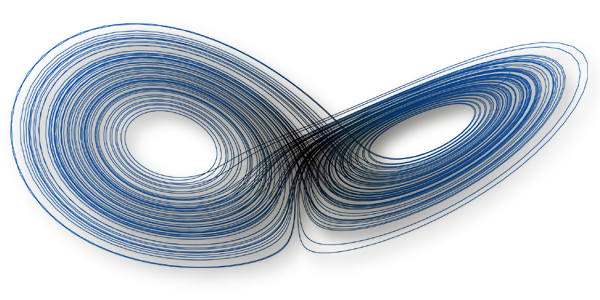
\includegraphics[width=.4\paperwidth]{cover.png}}

\date[unused]{ENSAM, Master 2, 2017--2018}

\begin{document}

\titleframe % Print the title as the first slide
%-------------------------------------------------------------------------------
%										Wiener Process
%-------------------------------------------------------------------------------

\begin{frame}[t, c]{}
	\centering
	\vspace{1cm}

	{\Large \textbf{Quick recap of statistics}}

	\bigskip

	{\textgre{\textbf{Basic concepts and definitions}}}

\end{frame}

\begin{frame}[t, c]{ACF and the Wiener-Khinchin theorem}{AutoCorrelation Function}
	\begin{itemize}
		\item Consider a time series $x(t)$. Assuming that this signal is known over an infinitely long interval $\left[ -T, T \right]$ (with $T \to \infty$), we can build the following function
		$$
			G(\tau) = \lim_{T \to \infty} \frac{1}{T} \int_0^T x(t) x(t+\tau) \ \mathrm{d}t
		$$
		known as the \emph{autocorrelation function} (ACF) of the signal $x(t)$.

		\medskip

		\item ACF is an even function. We often depict $G(\tau)$ for $\tau \ge 0$ only.

		\medskip

		\item It is a measure of how similar $x(t)$ and $x(t+\tau)$ are.
	\end{itemize}

	\vspace{1cm}
\end{frame}

\begin{frame}[t, c]{ACF and the Wiener-Khinchin theorem}{Example}
	\begin{minipage}{.48\textwidth}
		\begin{itemize}
			\item Consider the signal $x(t) = A \cos(\Omega t)$.

			\medskip

			\item Its ACF is given by
			$$
			G(\tau) = \lim_{T \to \infty} \frac{A^2}{T} \int_0^T \cos \left( \Omega t \right) \cos \left( \Omega (t + \tau) \right) \ \mathrm{d}t
			$$

			\item After some simplification, we obtain
			$$
			G(\tau) = \frac{A^2 \cos(\Omega \tau)}{2}.
			$$
		\end{itemize}
	\end{minipage}%
	\hfill
	\begin{minipage}{.48\textwidth}
		\centering
		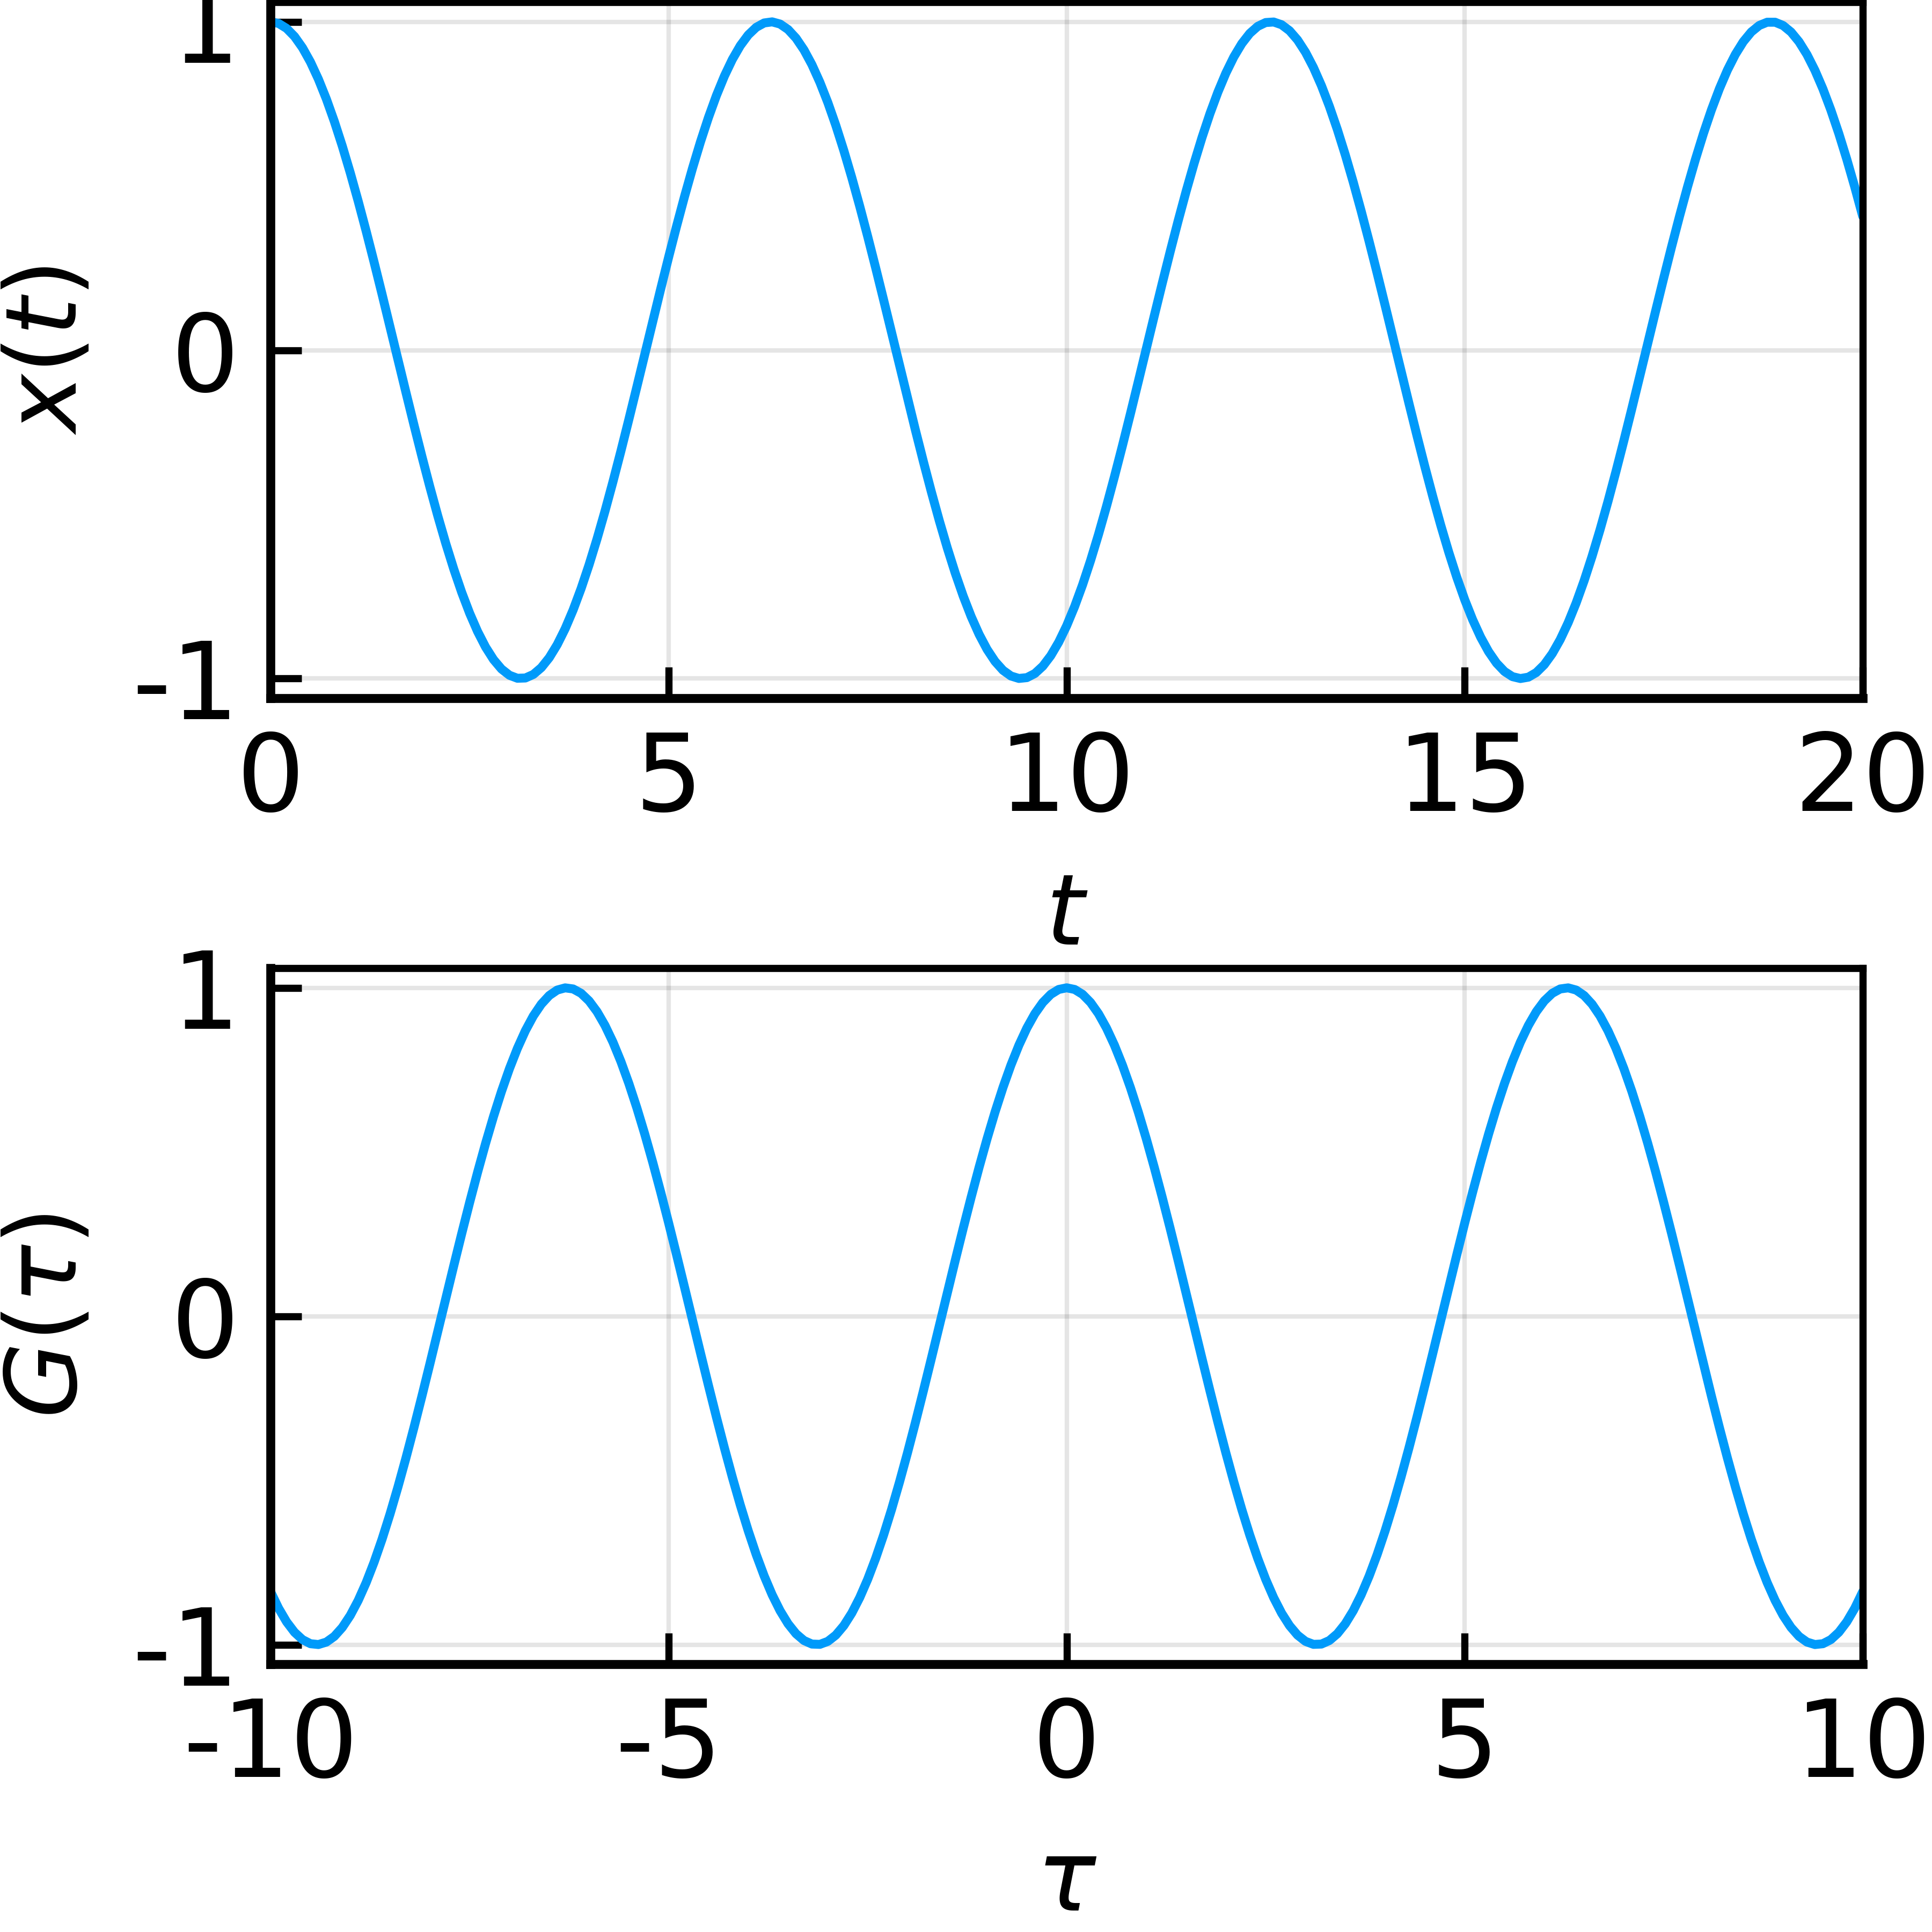
\includegraphics[width=.75\columnwidth]{cosine_acf}
	\end{minipage}

	\vspace{1cm}
\end{frame}

\begin{frame}[t, c]{ACF and the Wiener-Khinchin theorem}{Wiener-Khinchin theorem}
	\begin{itemize}
		\item Let us introduce the forward Fourier transform of $x(t)$
		$$
		\hat{x}(\omega) = \int_0^T x(t) e^{-i \omega t} \ \mathrm{d}t.
		$$

		\item The \emph{power spectral density} (PSD) of $x(t)$ is given by
		$$
		S(\omega) = \lim_{T \to \infty} \frac{1}{2\pi T} \vert \hat{x}(\omega) \vert^2.
		$$

		\item Wiener-Khinchin theorem states that ACF and PSD are related as follows
		$$
		G(\tau) = \int_{-\infty}^{\infty} S(\omega) e^{i \omega \tau} \ \mathrm{d}\omega.
		$$
		\begin{itemize}
			\item[$\hookrightarrow$] ACF is the inverse Fourier transform of PSD.
		\end{itemize}
	\end{itemize}

	\vspace{1cm}
\end{frame}

\begin{frame}[t, c]{ACF and the Wiener-Khinchin theorem}{Example}
	\begin{minipage}{.48\textwidth}
		\begin{itemize}
			\item Consider the signal $x(t) = A \cos(\Omega t)$.

			\medskip

			\item Its ACF is given by
			$$
			G(\tau) = \frac{A^2 \cos(\Omega \tau)}{2}.
			$$

			\item Its PSD is given by
			$$
			S(\omega) = \delta(\Omega - \omega).
			$$
		\end{itemize}
	\end{minipage}%
	\hfill
	\begin{minipage}{.48\textwidth}
		\centering
		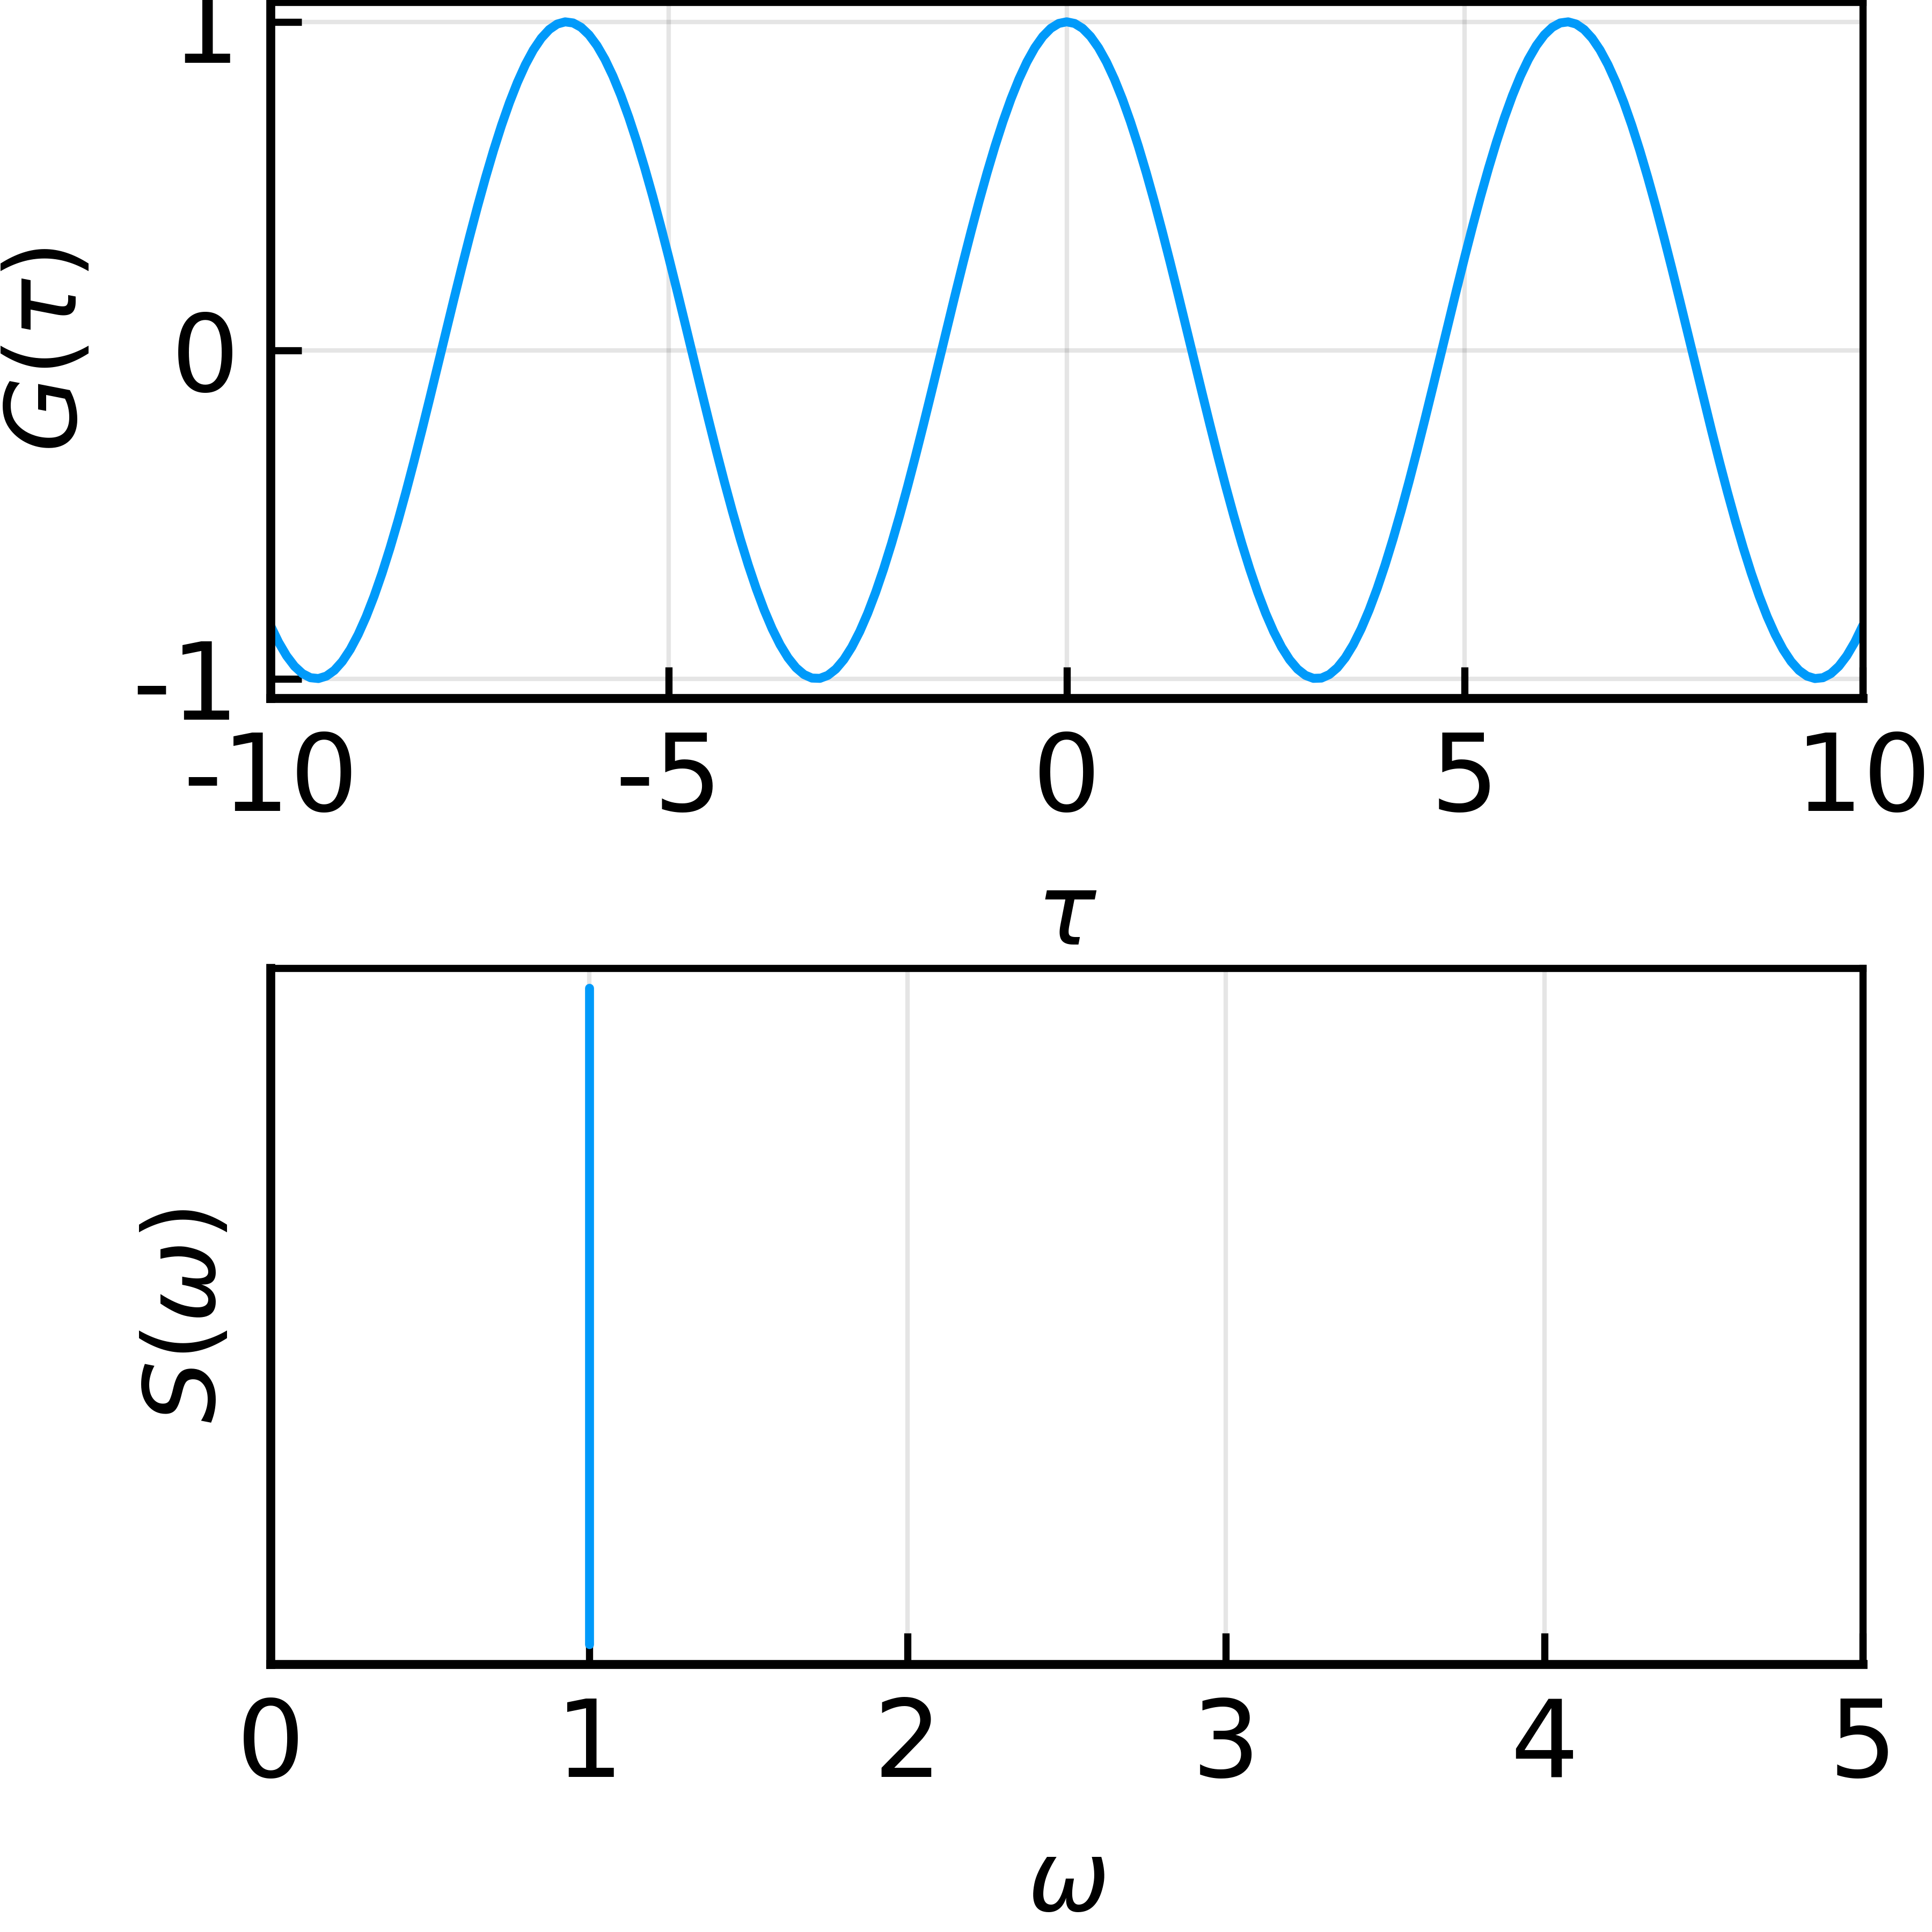
\includegraphics[width=.75\columnwidth]{cosine_acf_psd}
	\end{minipage}

	\vspace{1cm}
\end{frame}

\begin{frame}[t, c]{White noise}{Same excitation for all frequencies}
	\centering

	\begin{itemize}
		\item \emph{White noise} is a random signal having equal intensity at different frequencies.

		\medskip

		\item Various white noises can be generated depending on the distribution of the noise amplitude.
		\begin{itemize}
			\item[$\hookrightarrow$] Gaussian, Poisson, Laplace, Uniform, ...
		\end{itemize}
	\end{itemize}

	\bigskip

	
\includegraphics[width=.9\textwidth]{gaussian_white_noise} \\
	\textbf{Fig 1.:} Realization of a Gaussian white noise.

	\vspace{1cm}
\end{frame}

\begin{frame}[t, c]{White noise}{Gaussian white noise}
	\begin{minipage}{.48\textwidth}
		\begin{itemize}
			\item What most people really imply is \emph{Gaussian white noise}.
			\begin{itemize}
				\item[$\hookrightarrow$] Constant Power Spectral Density.
				\item[$\hookrightarrow$] $\delta$-correlated.
				\item[$\hookrightarrow$] Amplitude drawn from a normal distribution.
			\end{itemize}

			\item Makes a number of stochastic problems tractables from an analytical point of view.

			\medskip

			\item Numerous other types of white noise exist.
		\end{itemize}
	\end{minipage}%
	\hfill
	\begin{minipage}{.48\textwidth}
		\centering
		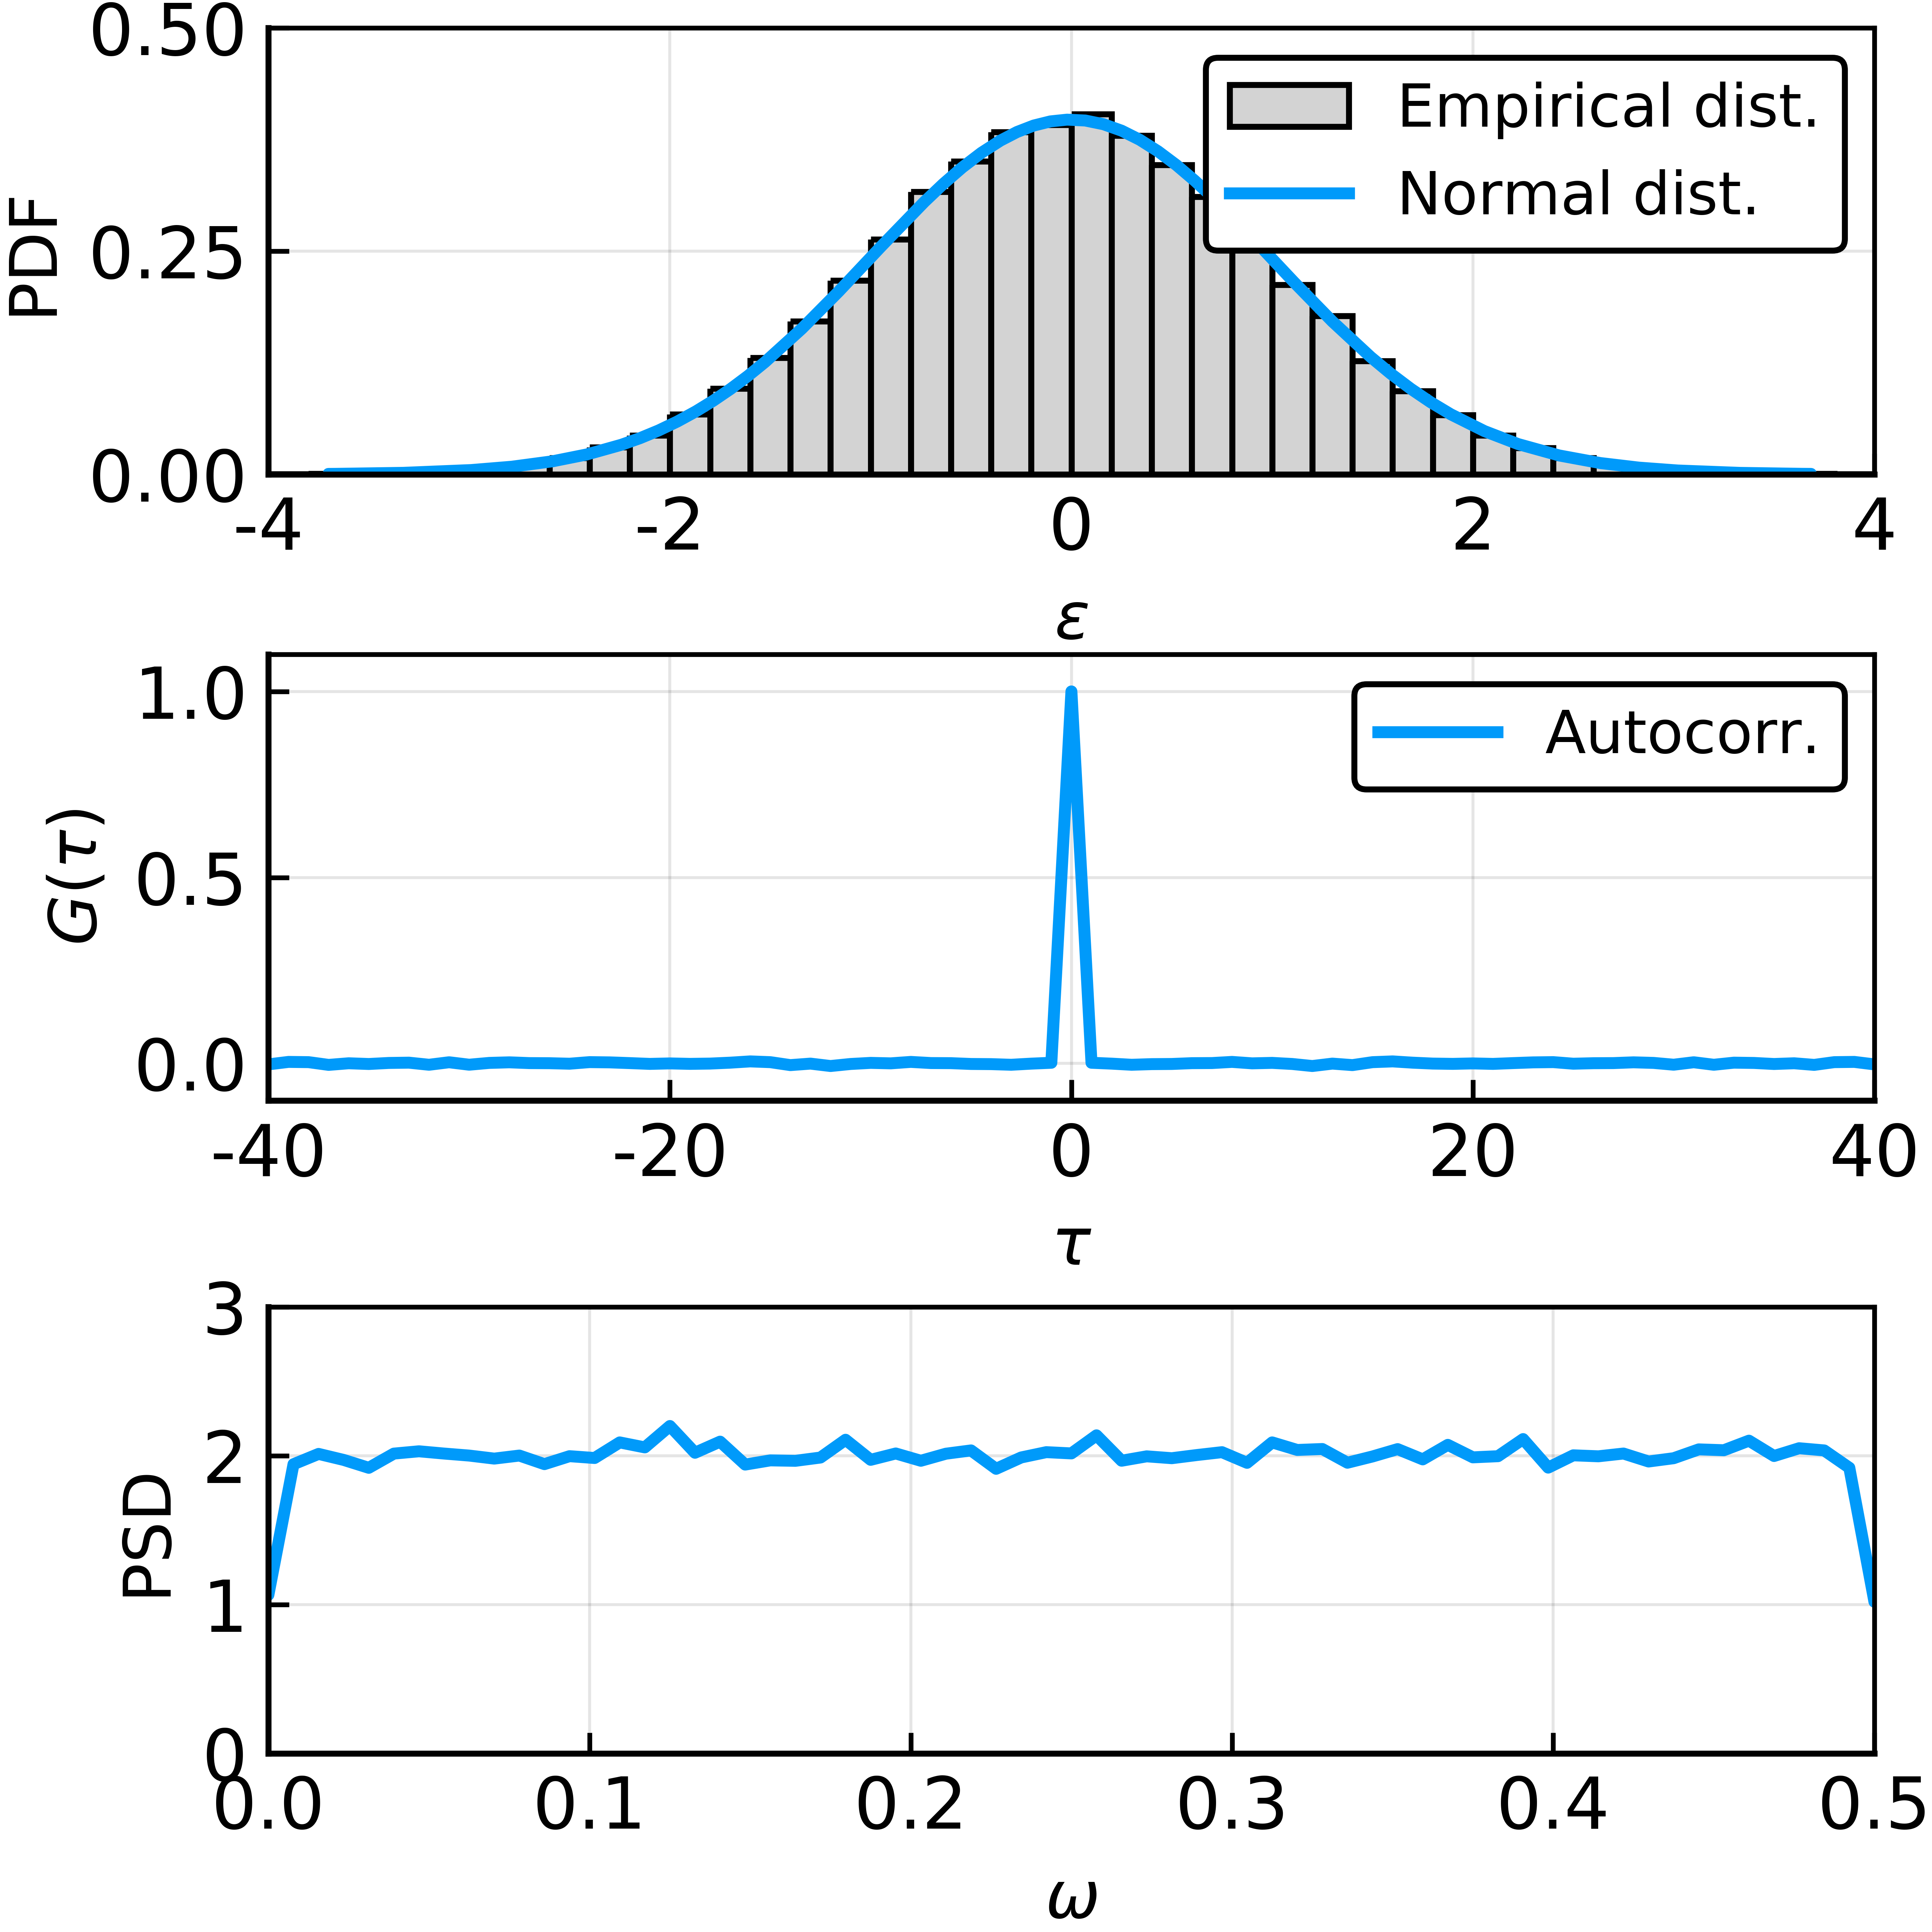
\includegraphics[width=.9\columnwidth]{gaussian_white_noise_total}
	\end{minipage}

	\vspace{1cm}
\end{frame}

\begin{frame}[t, c]{White noise}{Examples}
	\centering

	
\includegraphics[width=.8\textwidth]{gaussian_white_noise}


	
\includegraphics[width=.8\textwidth]{uniform_white_noise}


	
\includegraphics[width=.8\textwidth]{laplace_white_noise}

	\vspace{1cm}
\end{frame}

\begin{frame}[t, c]{White noise}{Examples}
	\begin{minipage}{.32\textwidth}
		\centering

		\textbf{Gaussian}

		\bigskip

		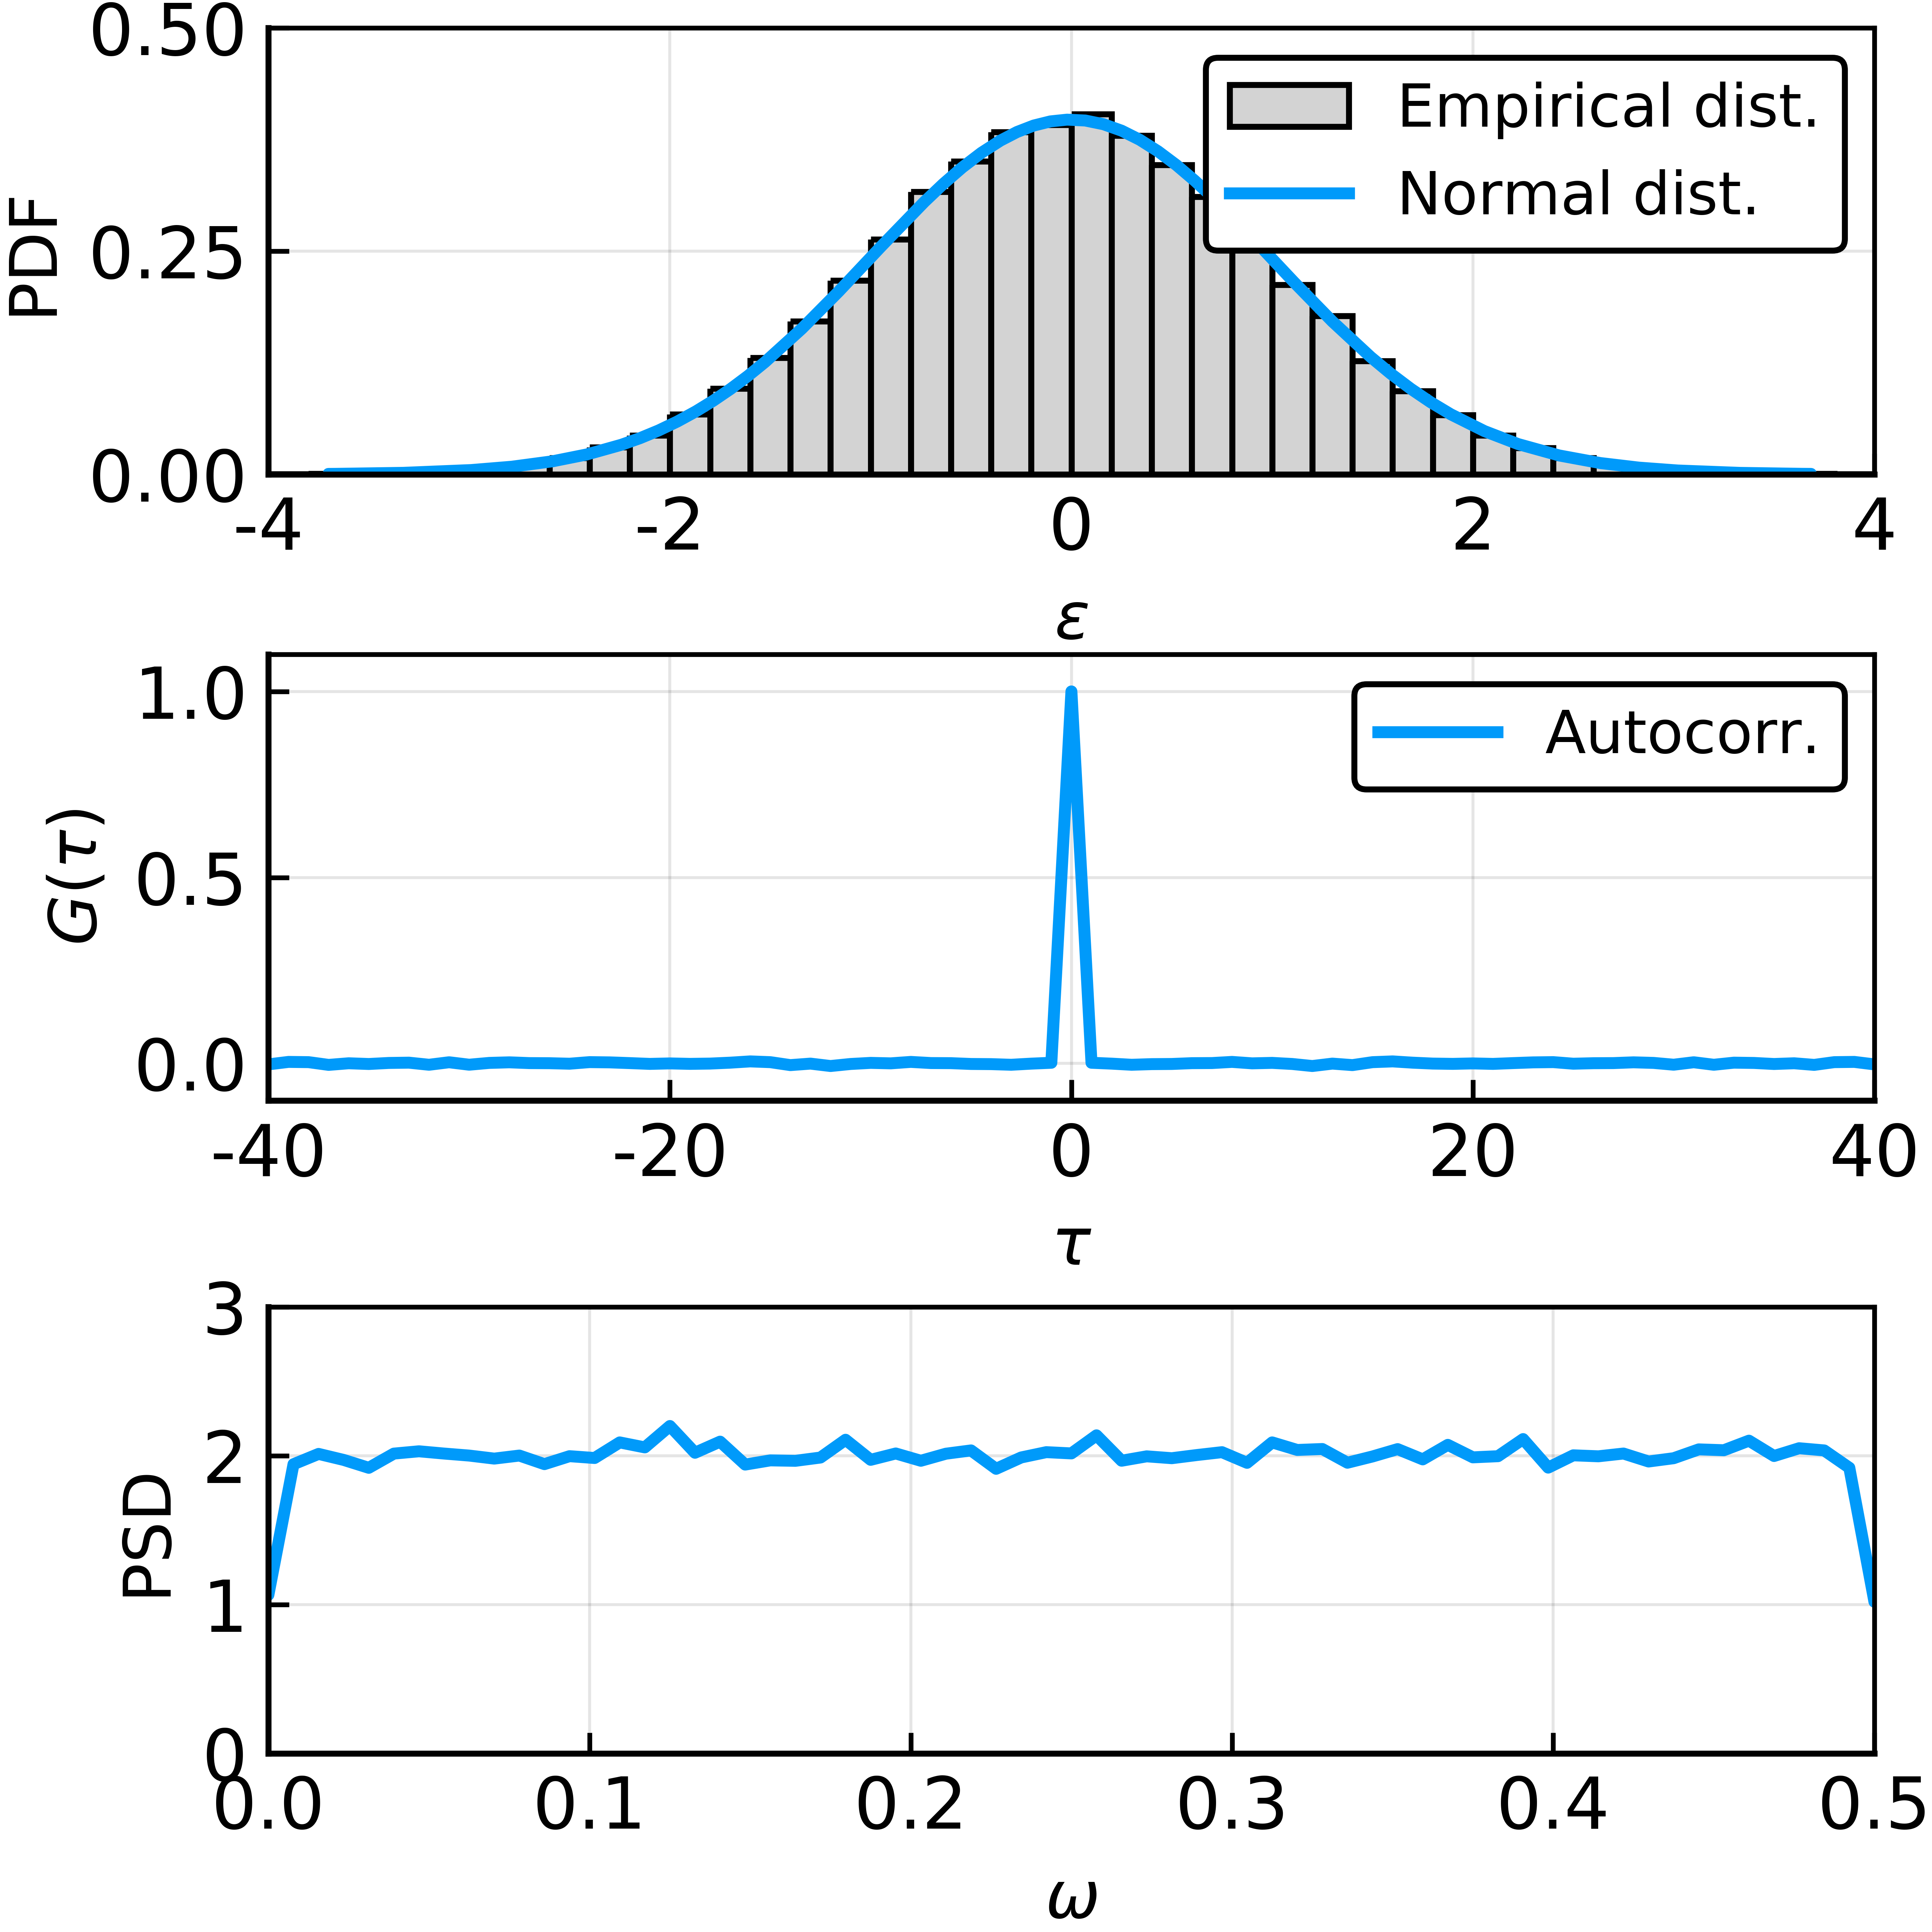
\includegraphics[width=\textwidth]{gaussian_white_noise_total}
	\end{minipage}%
	\hfill
	\begin{minipage}{.32\textwidth}
		\centering

		\textbf{Uniform}

		\bigskip

		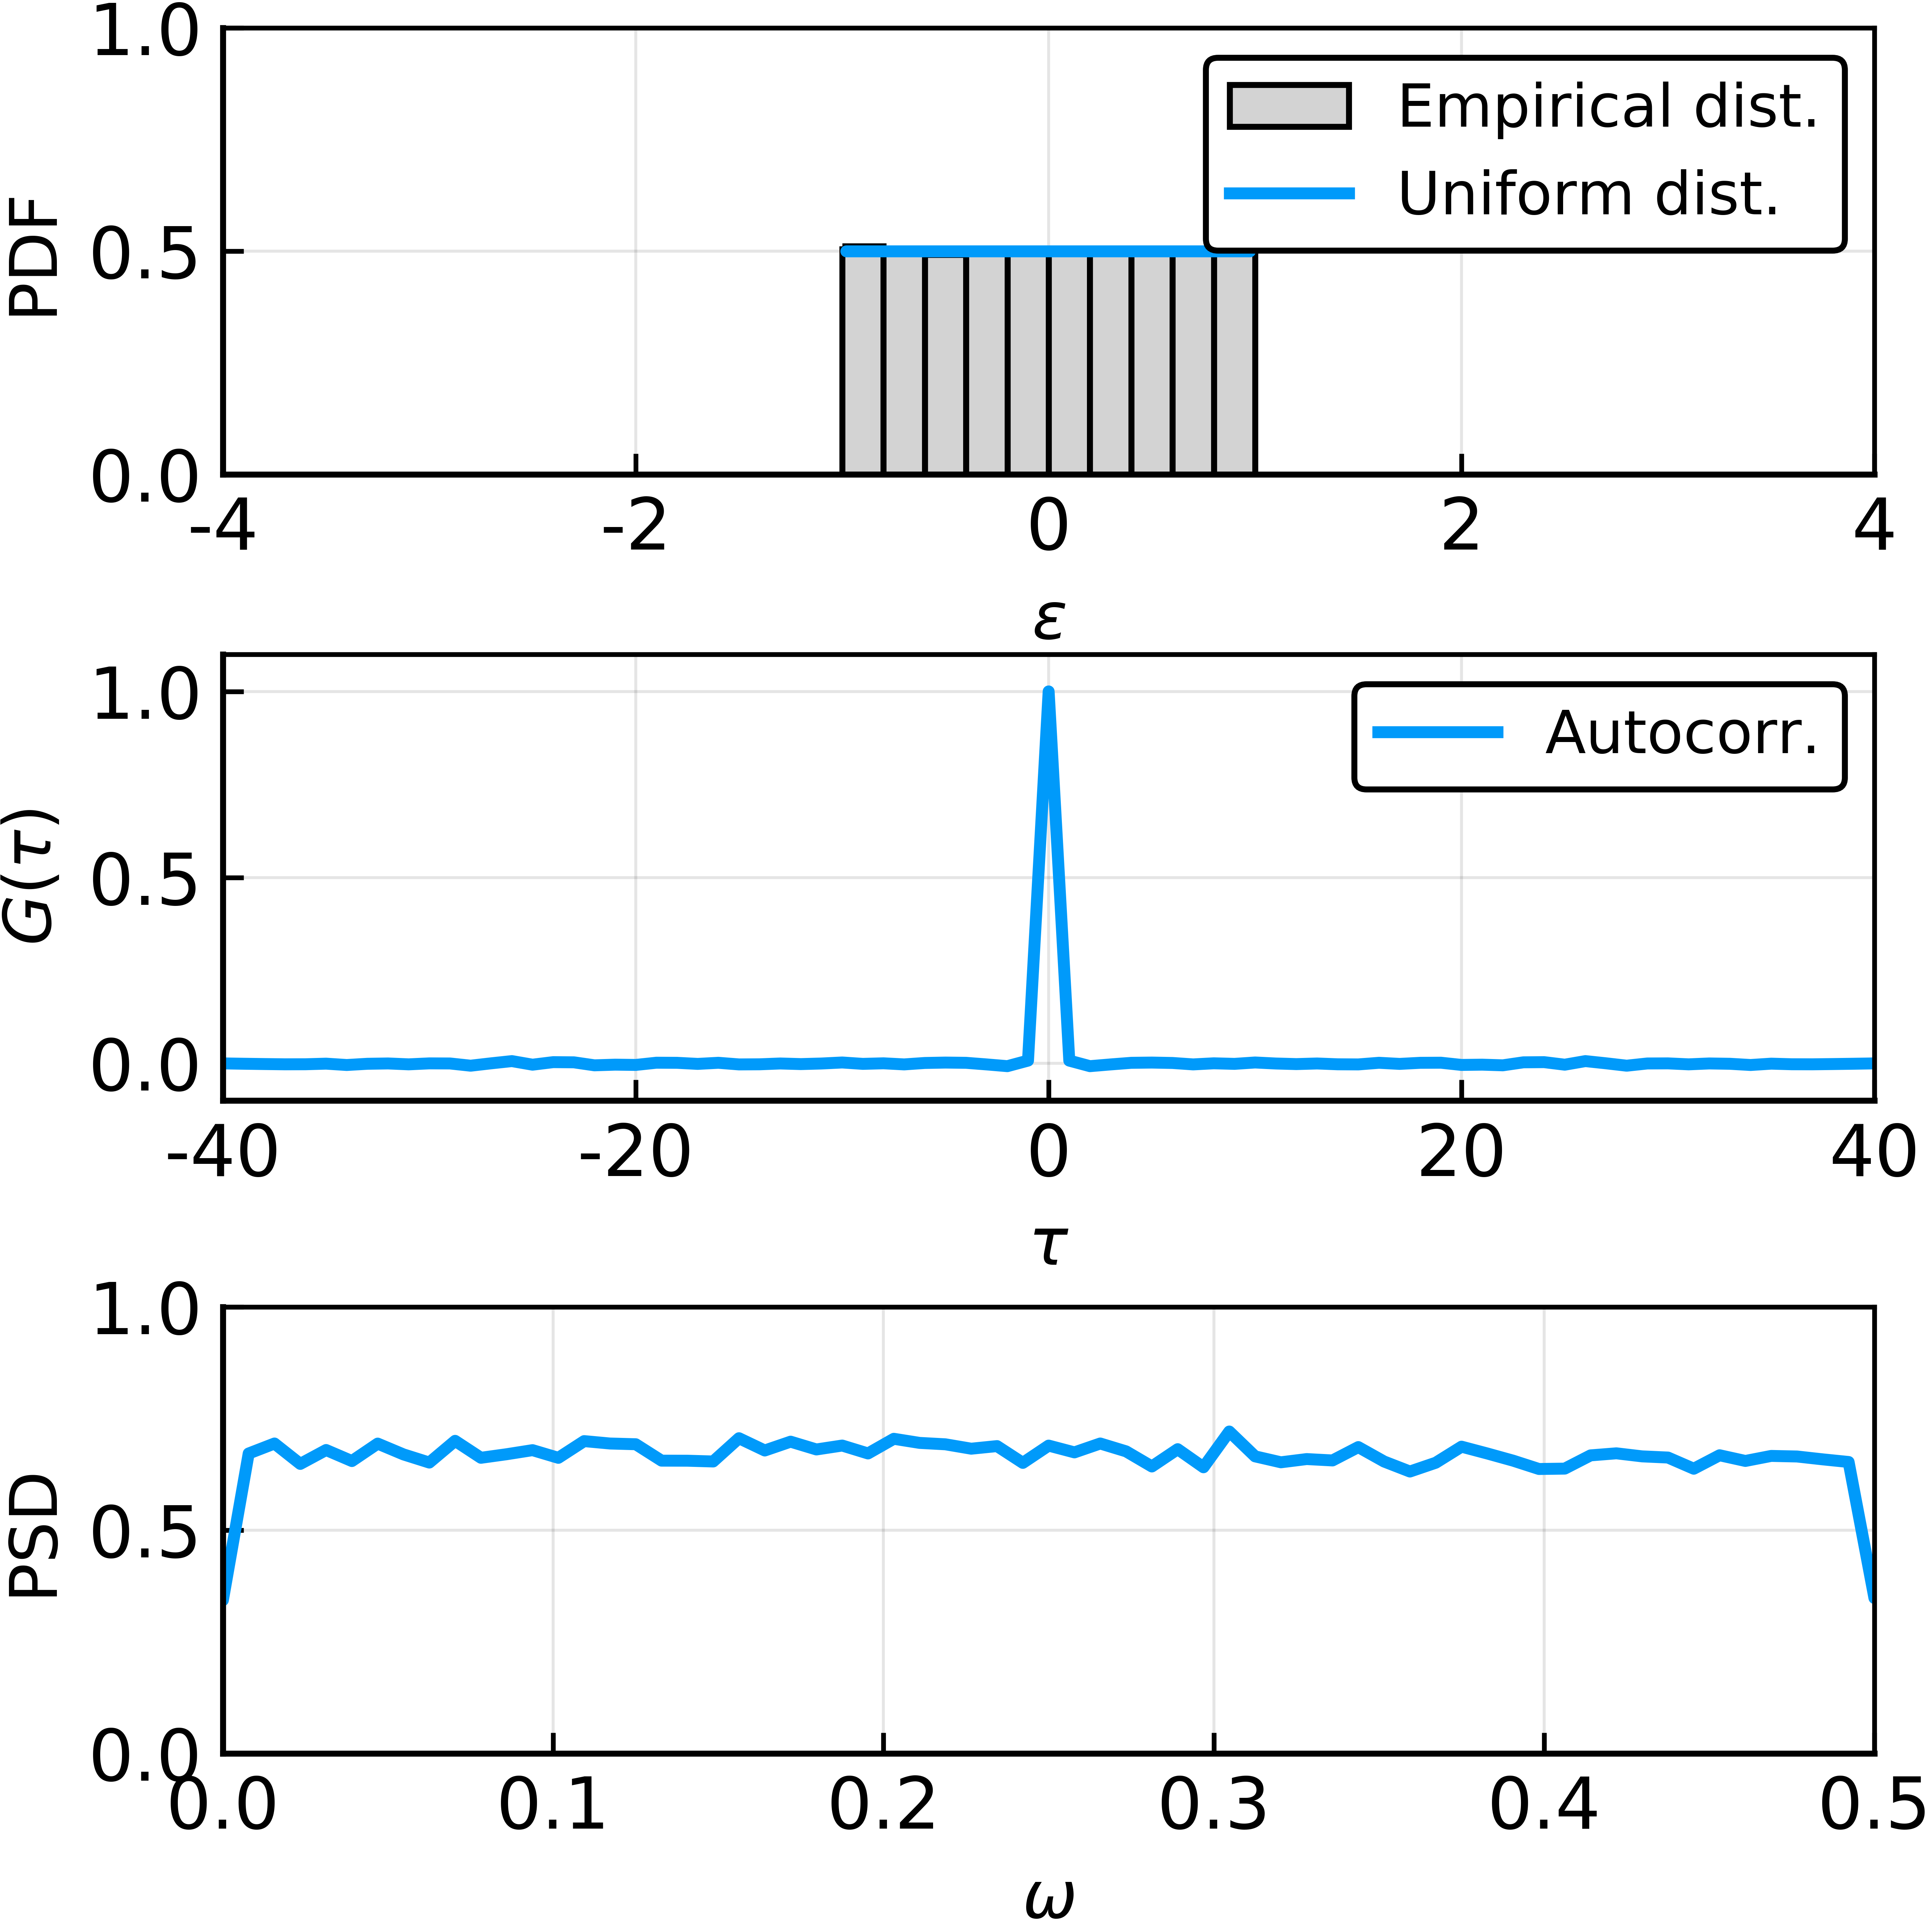
\includegraphics[width=\textwidth]{uniform_white_noise_total}
	\end{minipage}%
	\hfill
	\begin{minipage}{.32\textwidth}
		\centering

		\textbf{Laplace}

		\bigskip

		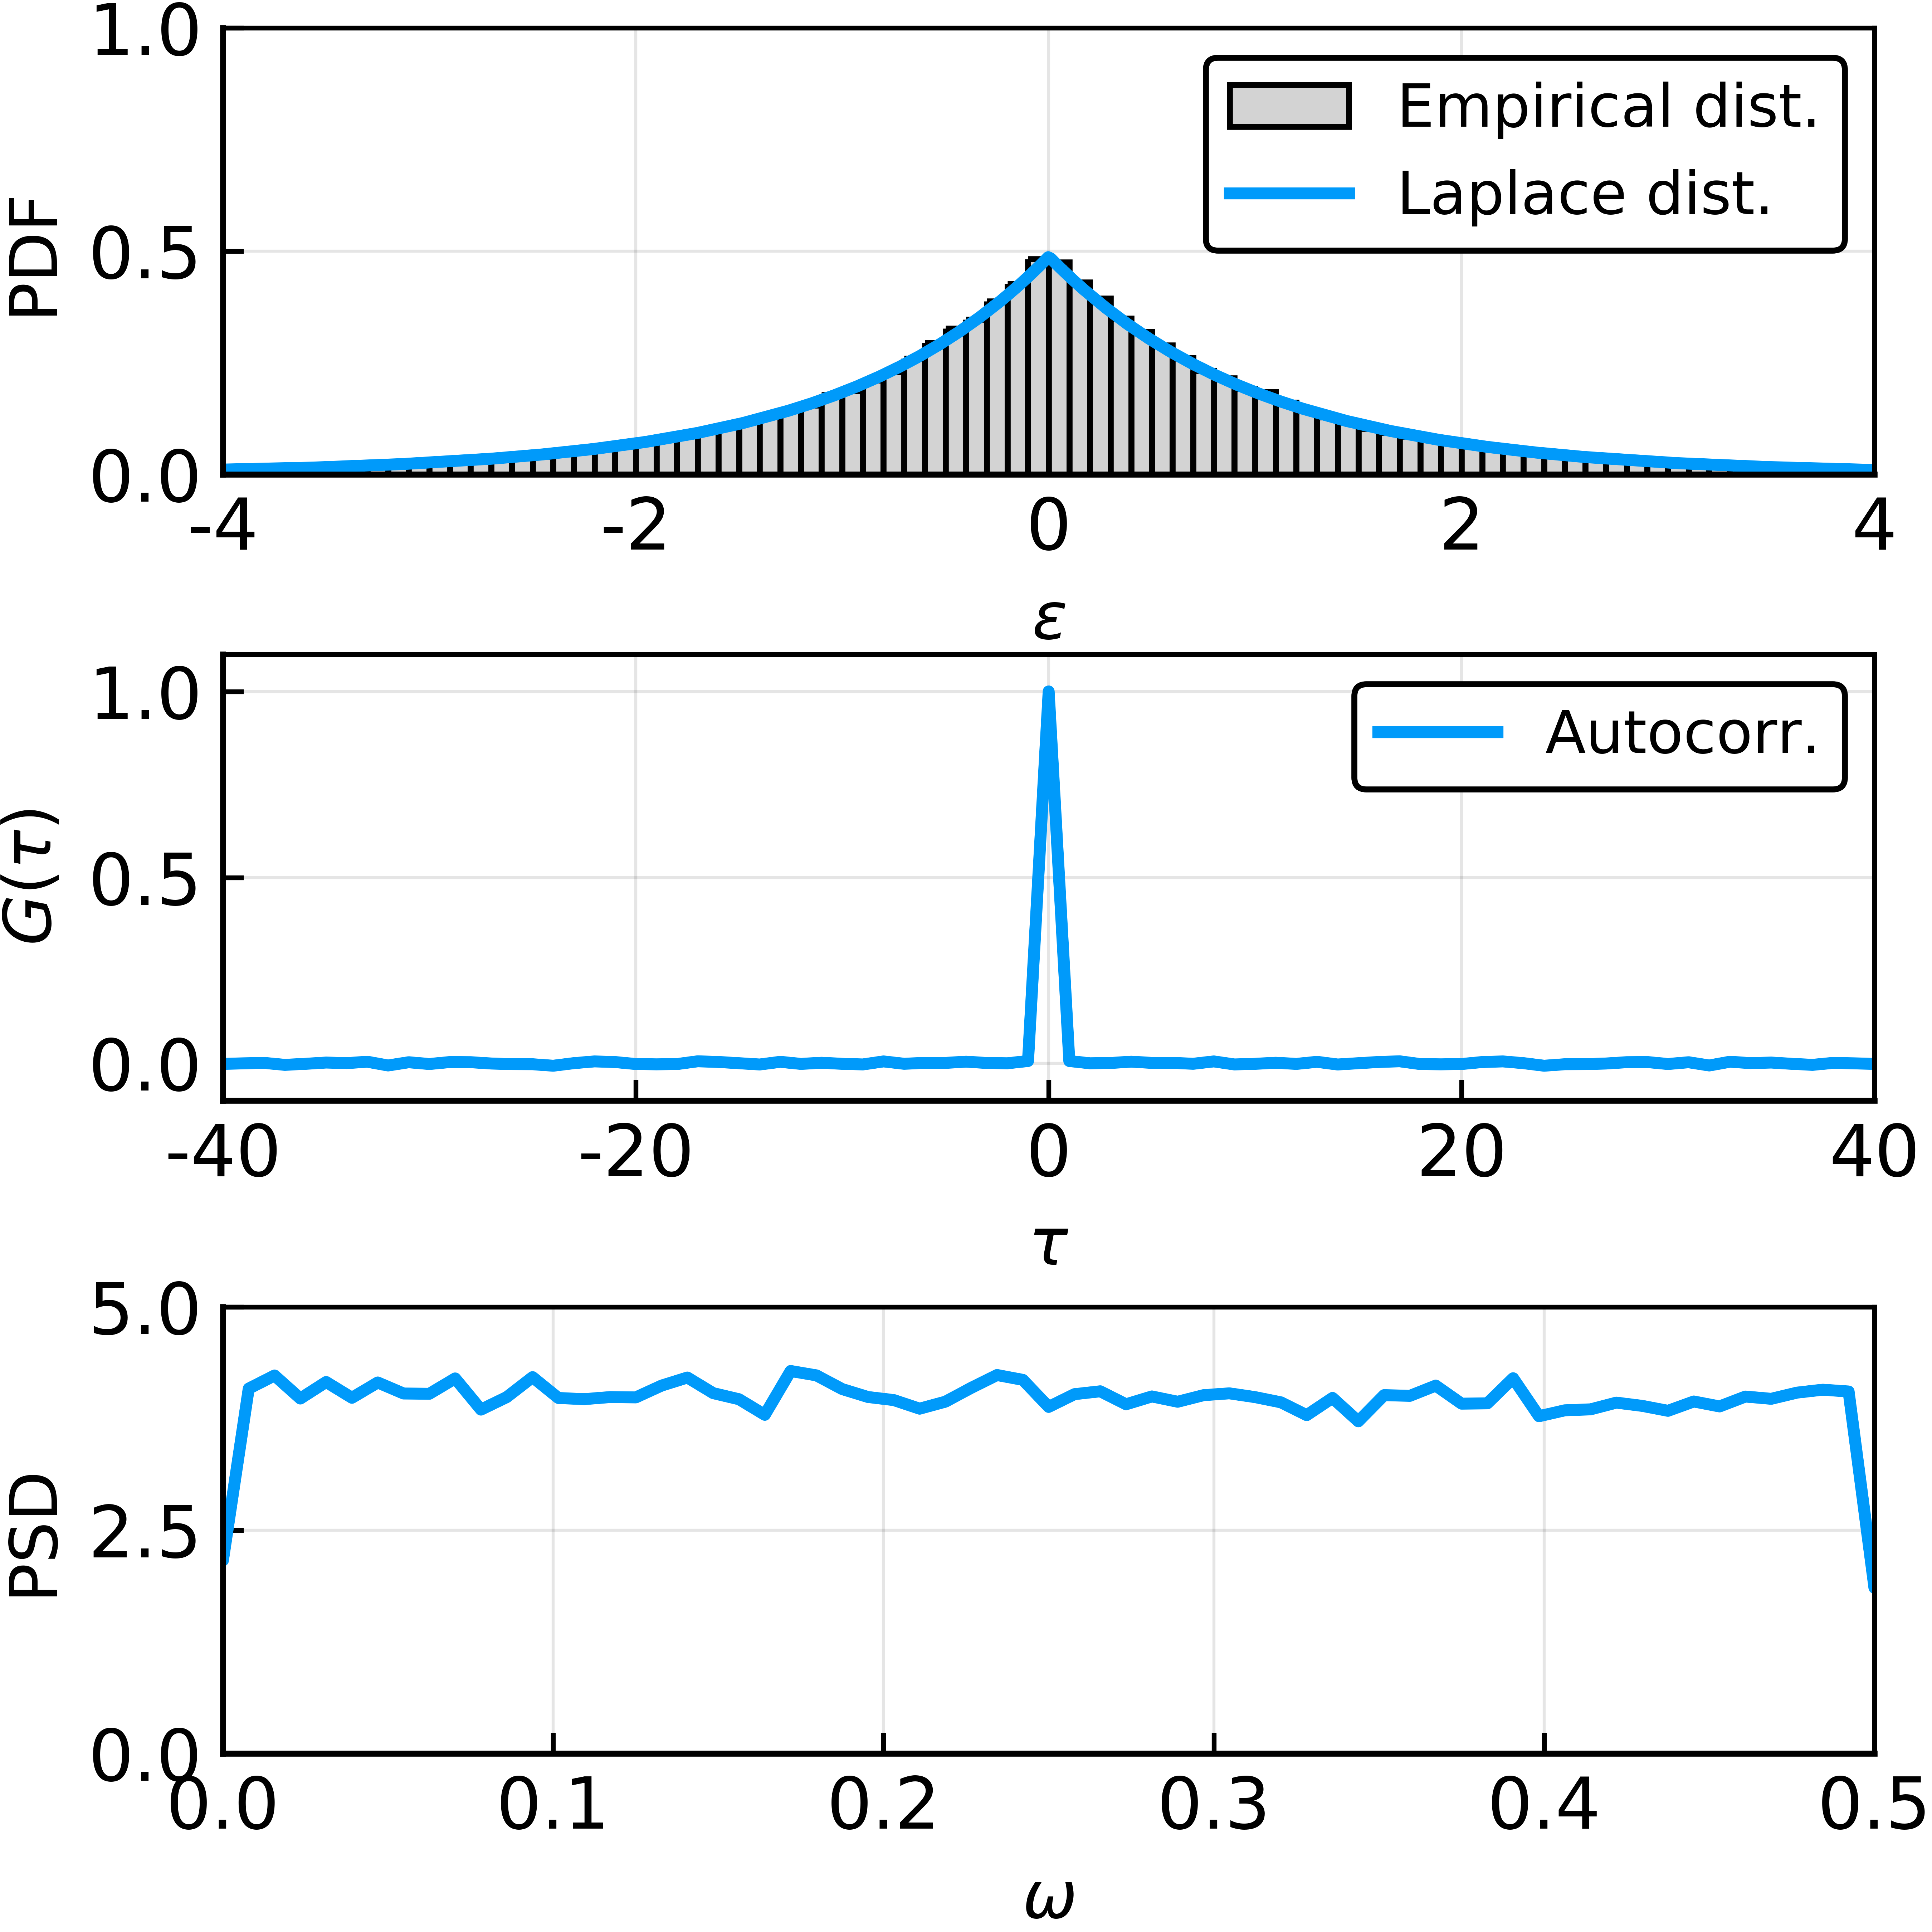
\includegraphics[width=\textwidth]{laplace_white_noise_total}
	\end{minipage}

	\vspace{1cm}
\end{frame}

%-------------------------------------------------------------------------------
%										Wiener Process
%-------------------------------------------------------------------------------

\begin{frame}[t, c]{}
	\centering
	\vspace{1cm}

	{\Large \textbf{Wiener Process}}

	\bigskip

	{\textgre{\textbf{The building block of stochastic dynamics}}}

\end{frame}

\begin{frame}[t, c]{Wiener Process}{Building block of stochastic dynamics}
	\begin{itemize}
		\item Wiener process satisfies the following Langevin equation
		$$
		\dot{x} = \eta
		$$
		where $\eta \sim \mathcal{N}(0, 1)$, i.e.\ a Gaussian white noise with zero-mean and unit-variance.
	\end{itemize}

	\vspace{1cm}
\end{frame}

\begin{frame}[t, c]{Wiener Process}{Monte-Carlo simualtions}
	\centering
	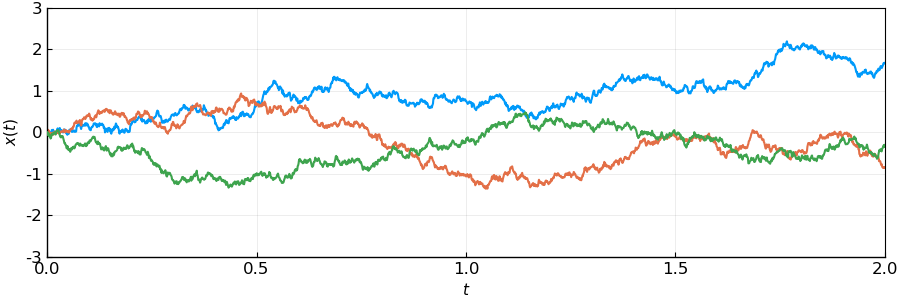
\includegraphics[width=.8\textwidth]{wiener_processes}

	\textbf{Fig. 1:} Three different realizations of the Wiener process.

	\vspace{1cm}
\end{frame}

\begin{frame}[t, c]{Wiener Process}{Monte-Carlo simualtions}
	\centering
	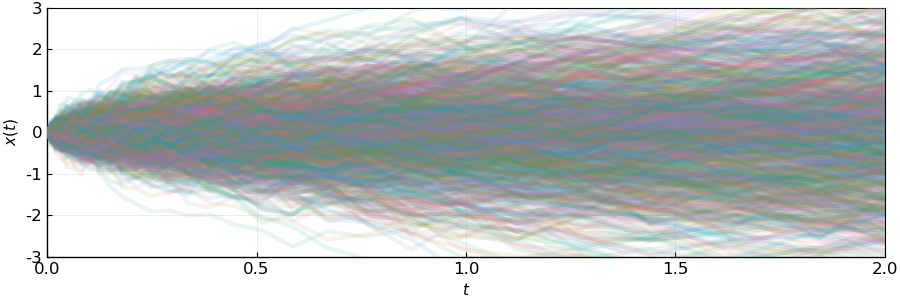
\includegraphics[width=.8\textwidth]{wiener_process_monte_carlo}

	\textbf{Fig. 2:} One hundred different realizations of the Wiener process.

	\vspace{1cm}
\end{frame}

\begin{frame}[t, c]{Wiener Process}{Monte-Carlo simualtions}
	\centering
	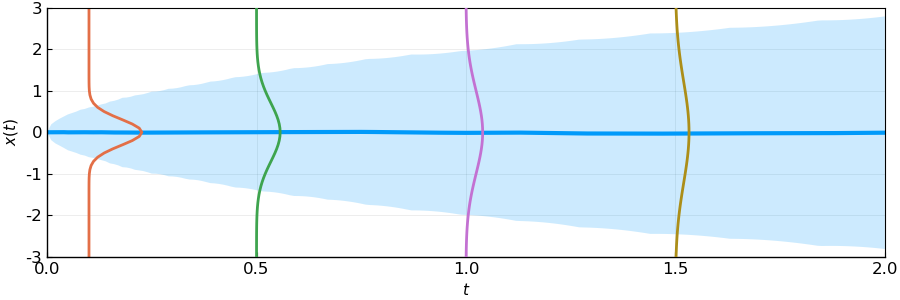
\includegraphics[width=.8\textwidth]{wiener_process_monte_carlo_summary}

	\textbf{Fig. 3:} Evolution of the probability density function.

	\vspace{1cm}
\end{frame}

\begin{frame}[t, c]{Wiener Process}{Fokker-Planck equation}
	\begin{minipage}{.48\textwidth}
		\begin{itemize}
			\item The Fokker-Planck equation reads
			$$
			\frac{\partial p}{\partial t} = \frac{1}{2} \frac{\partial^2 p}{\partial x^2}
			$$
			where $p(x, t)$ is the probability density function.

			\medskip

			\item It describes the diffusion of the PDF in phase space due to the stochastic term.

			\medskip

			\item If $p(x, 0) = \delta(x)$, then
			$$
			p(x, t) = \frac{1}{\sqrt{2 \pi t}} e^{-x^2 / (2t)}.
			$$
		\end{itemize}
	\end{minipage}%
	\hfill
	\begin{minipage}{.48\textwidth}
		\centering
		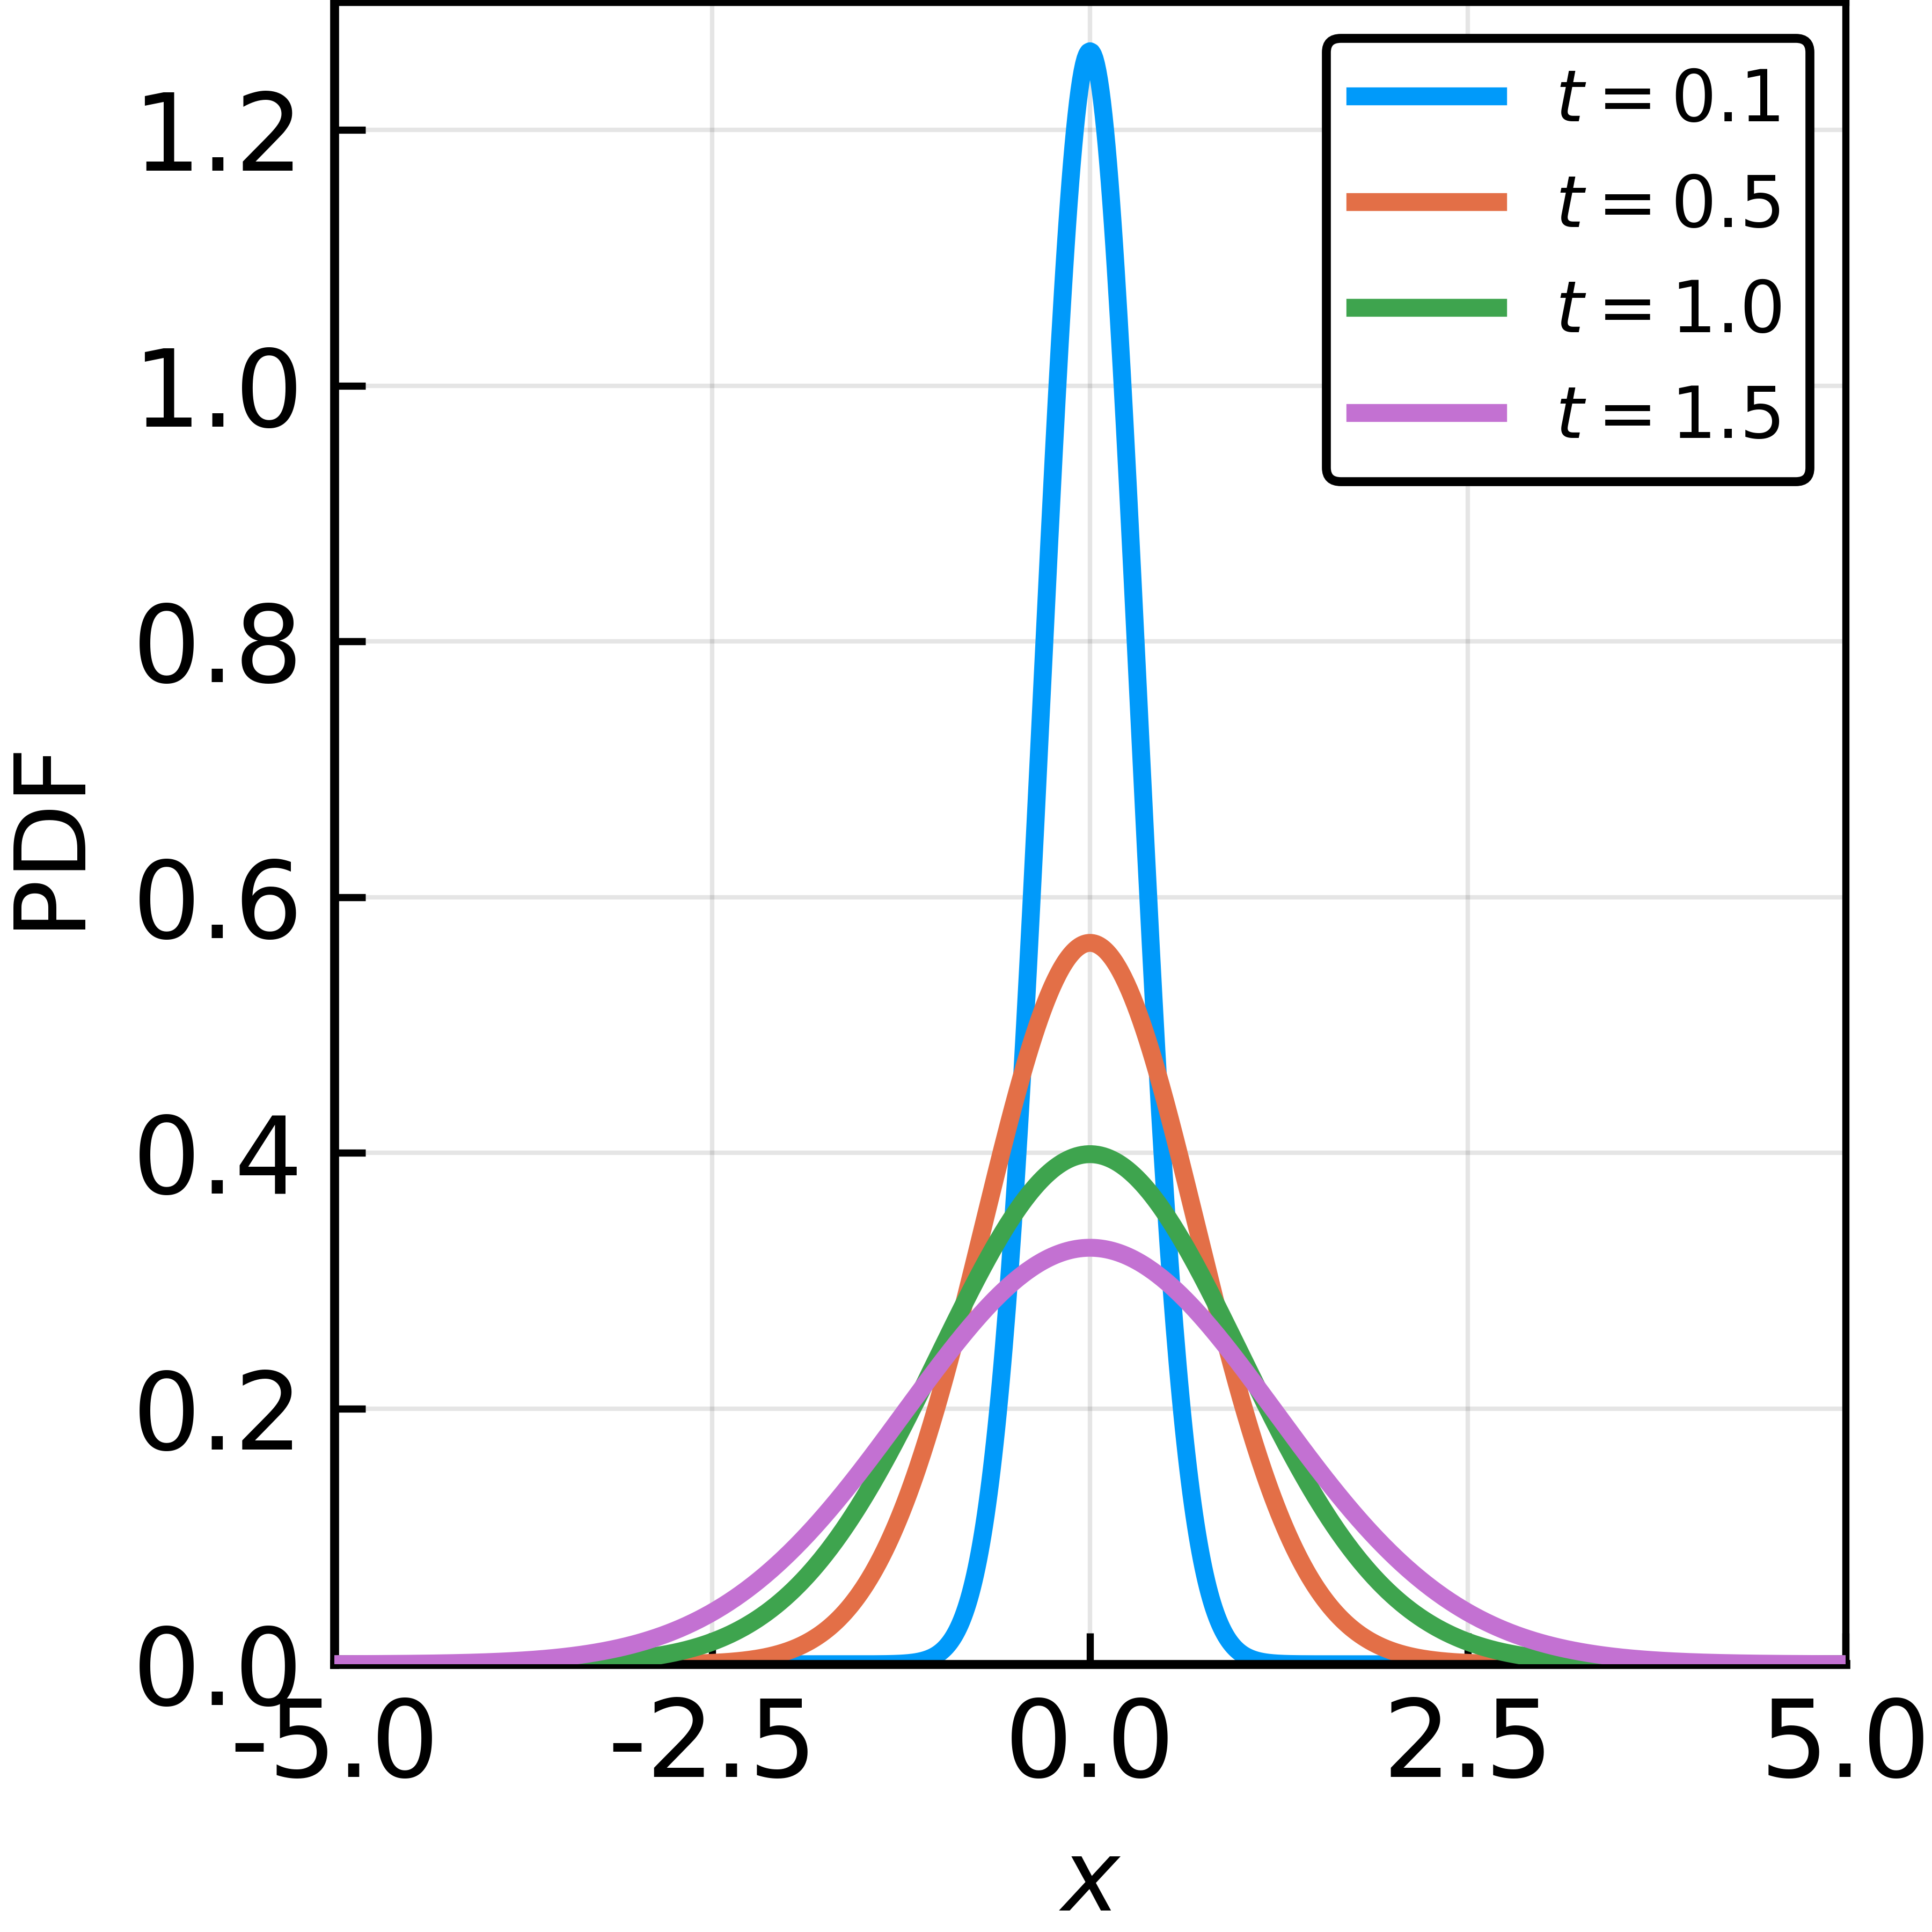
\includegraphics[width=.75\columnwidth]{wiener_process_pdf}

		\small{
			\textbf{Fig. 4:} Time-dependent PDF of the Wiener process.
			}
	\end{minipage}

	\vspace{1cm}
\end{frame}

%-------------------------------------------------------------------------------
%										Ornstein-Uhlenbeck Process
%-------------------------------------------------------------------------------

\begin{frame}[t, c]{}
	\centering
	\vspace{1cm}

	{\Large \textbf{Ornstein-Uhlenbeck Process}}

	\bigskip

	{\textgre{\textbf{Noisy relaxation process}}}

\end{frame}

\begin{frame}[t, c]{Ornstein-Uhlenbeck process}{Noisy relaxation process}
	\begin{itemize}
		\item The Ornstein-Uhlenbeck process satistifes the following Langevin equation
		$$
		\dot{x} = \theta \left( \mu - x \right) + \sigma \eta
		$$
		with once again $\eta \sim \mathcal{N}(0, 1)$. We furthermore have $\theta > 0$ and $\sigma > 0$.

		\medskip

		\item It is a prototype of noisy relaxation process. It also describes the velocity of a massive Brownian particle under the influence of friction.
	\end{itemize}

	\vspace{1cm}
\end{frame}

\begin{frame}[t, c]{Ornstein-Uhlenbeck Process}{Monte-Carlo simualtions}
	\centering
	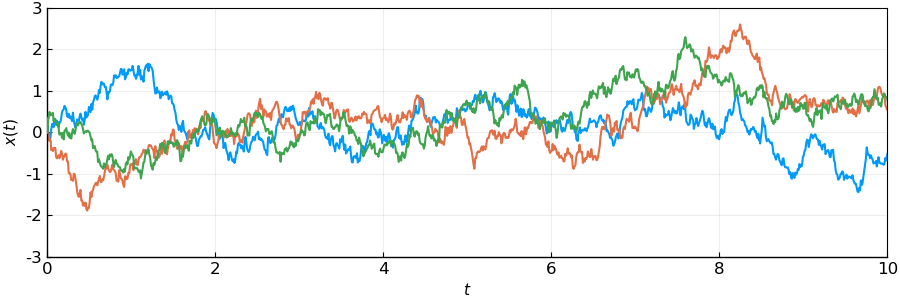
\includegraphics[width=.8\textwidth]{orstein_uhlenbeck_processes}

	\textbf{Fig. 1:} Three different realizations of the Wiener process.

	\vspace{1cm}
\end{frame}

\begin{frame}[t, c]{Ornstein-Uhlenbeck Process}{Monte-Carlo simualtions}
	\centering
	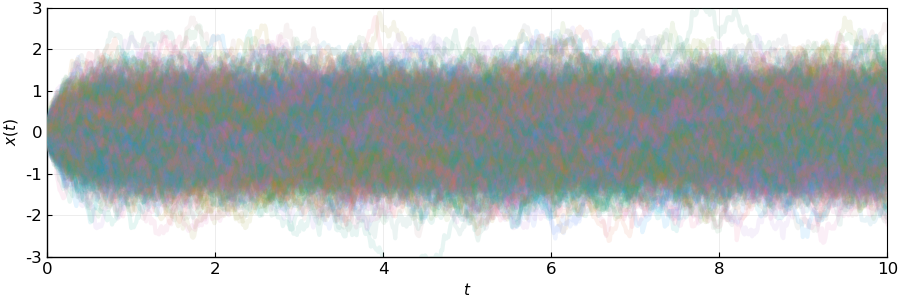
\includegraphics[width=.8\textwidth]{orstein_uhlenbeck_process_monte_carlo}

	\textbf{Fig. 2:} One hundred different realizations of the Wiener process.

	\vspace{1cm}
\end{frame}

\begin{frame}[t, c]{Ornstein-Uhlenbeck Process}{Monte-Carlo simualtions}
	\centering
	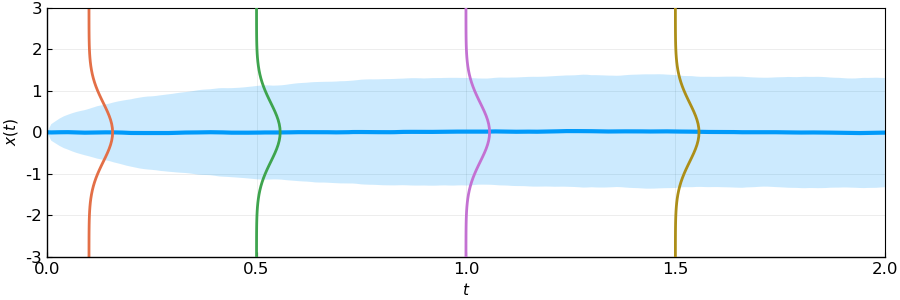
\includegraphics[width=.8\textwidth]{orstein_uhlenbeck_process_monte_carlo_summary}

	\textbf{Fig. 3:} Evolution of the probability density function.

	\vspace{1cm}
\end{frame}

\begin{frame}[t, c]{Ornstein-Uhlenbeck Process}{Fokker-Planck equation}
	\begin{minipage}{.48\textwidth}
		\begin{itemize}
			\item The Fokker-Planck equation reads
			$$
			\frac{\partial p}{\partial t} = \theta \frac{\partial}{\partial x} \left[ \left( x - \mu \right) p \right] + \frac{\sigma^2}{2} \frac{\partial^2 p}{\partial x^2}
			$$
			where $p(x, t)$ is the probability density function.

			\medskip

			\item Its stationnary solution reads
			$$
			p(x) = \sqrt{\frac{\theta}{\pi \sigma^2}} e^{-\theta (x - \mu)^2 / \sigma^2}.
			$$
		\end{itemize}
	\end{minipage}%
	\hfill
	\begin{minipage}{.48\textwidth}
		\centering
		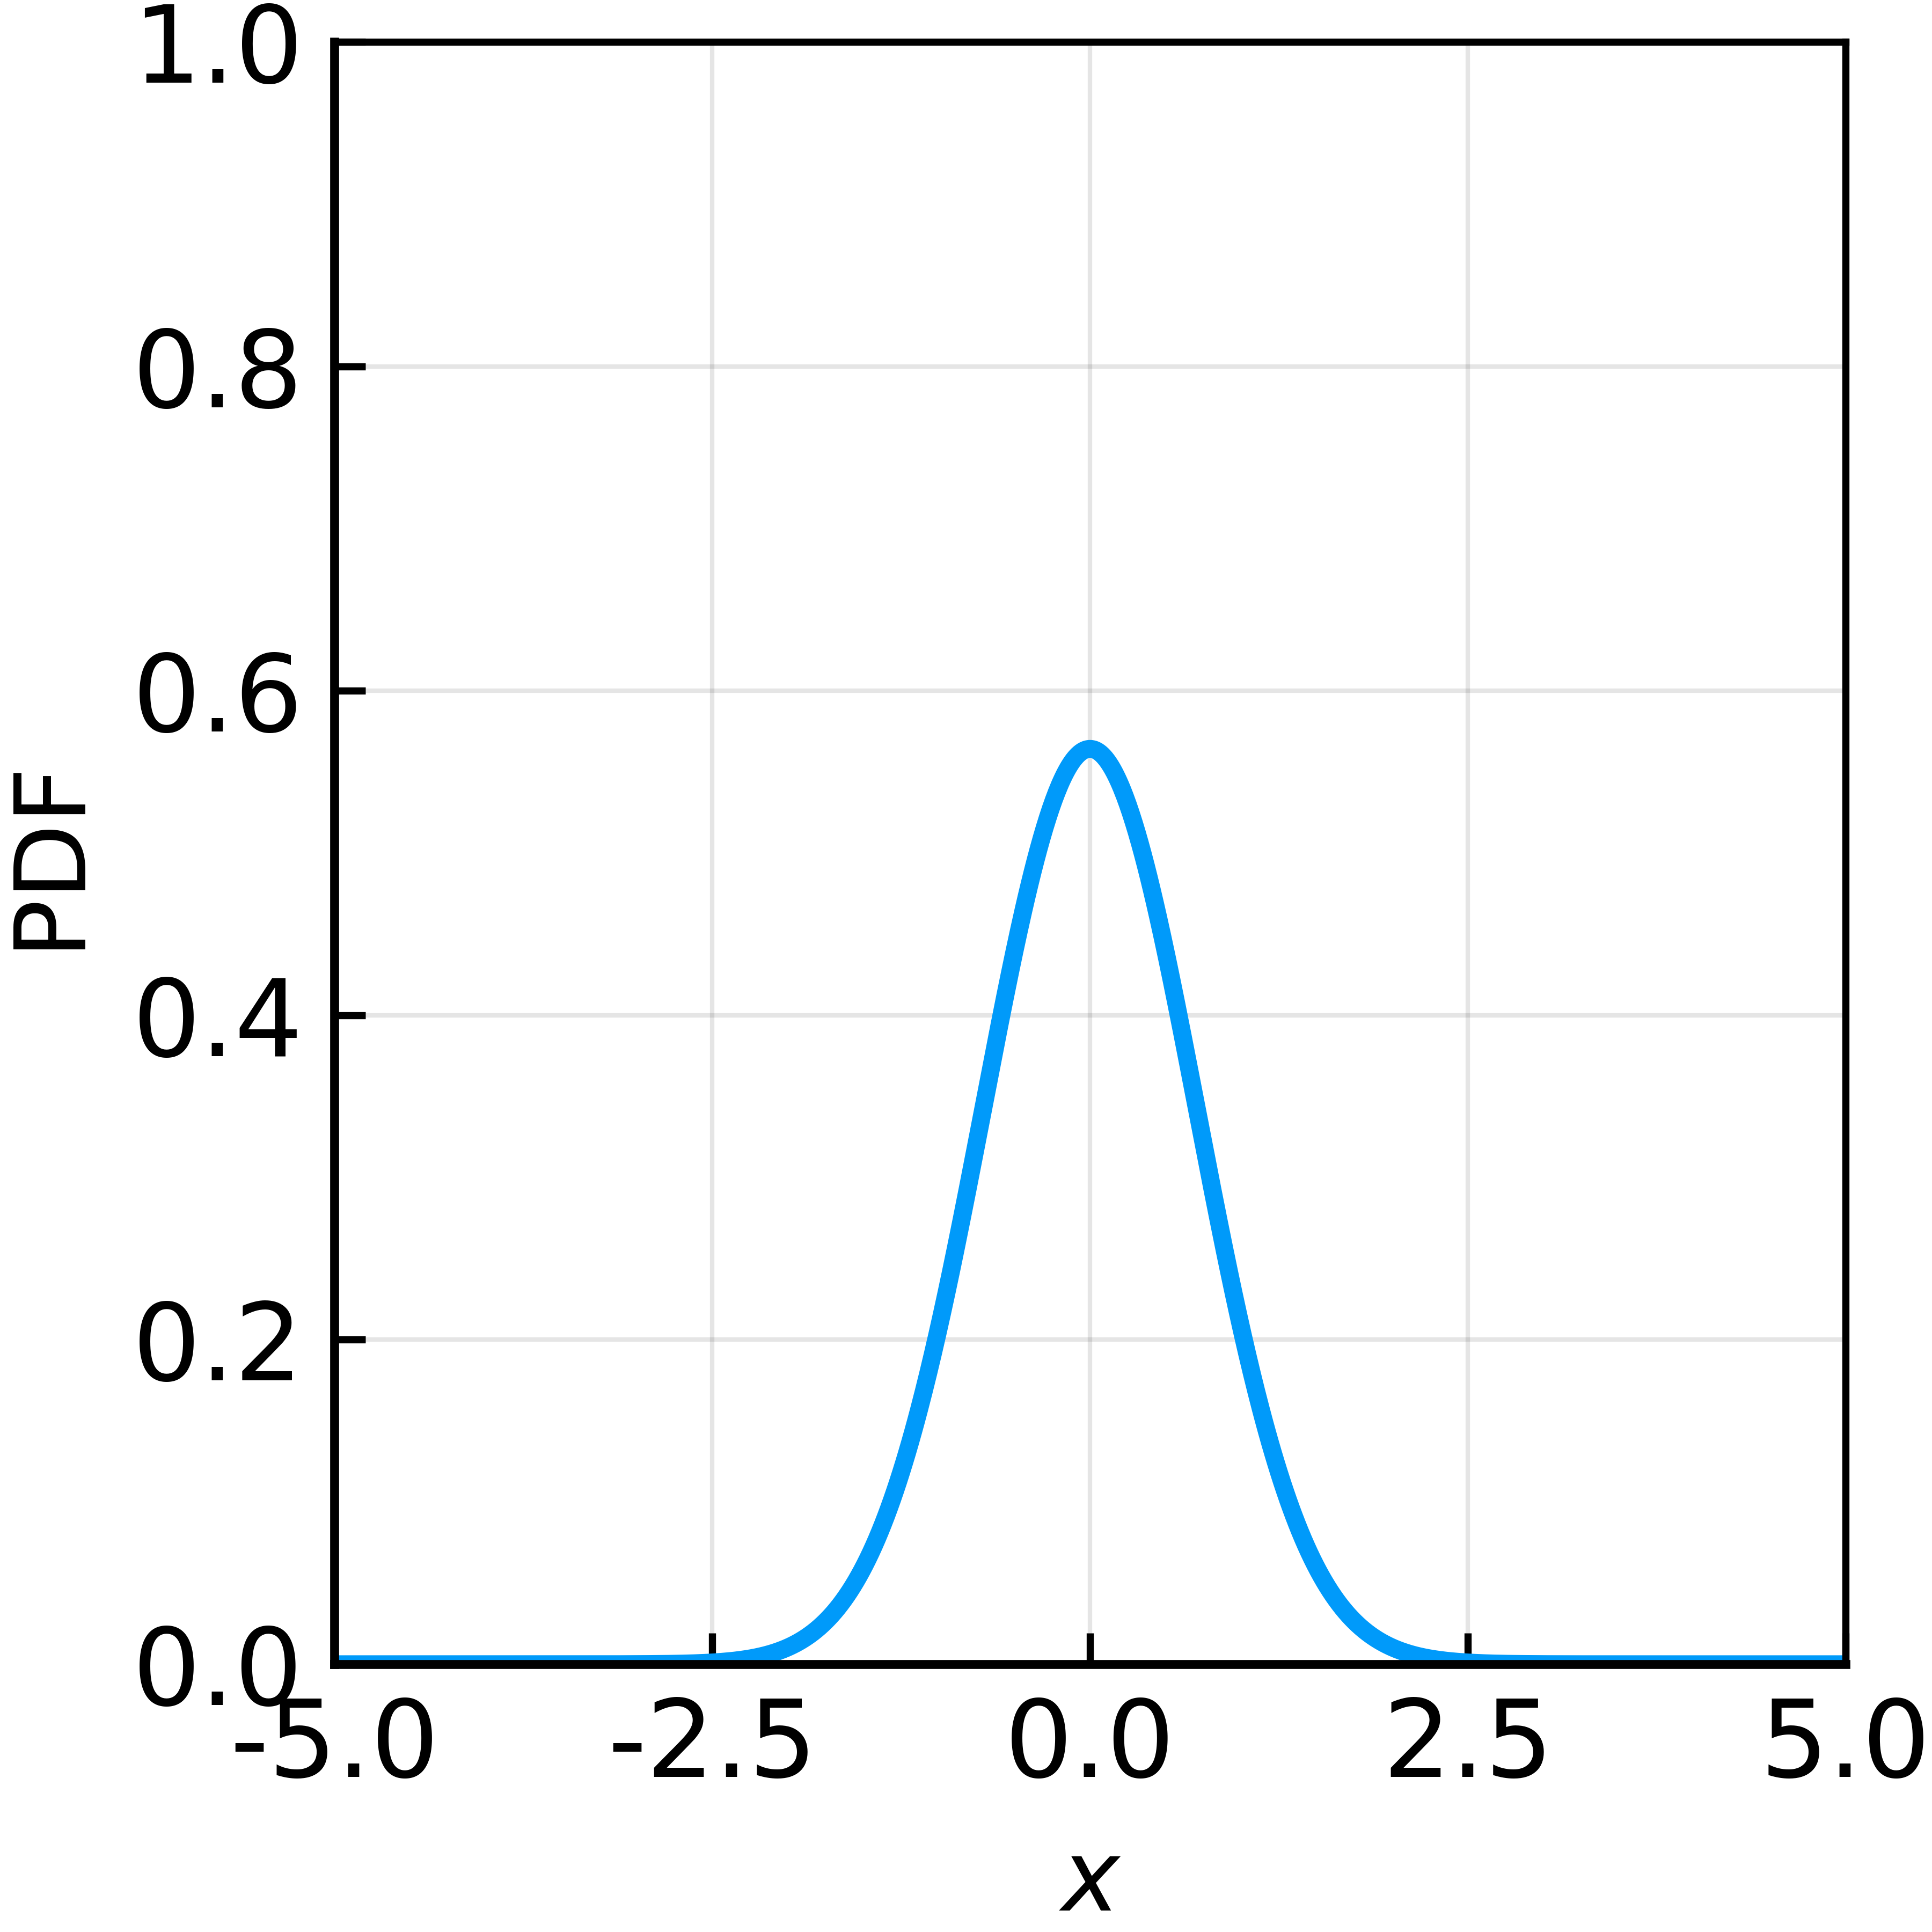
\includegraphics[width=.75\columnwidth]{ornstein_uhlenbeck_process_pdf}

		\small{
			\textbf{Fig. 4:} Stationnary PDF of the OU process.
			}
	\end{minipage}

	\vspace{1cm}
\end{frame}

\begin{frame}[t, c]{Ornstein-Uhlenbeck Process}{Power Spectral Density}
	\begin{minipage}{.48\textwidth}
		\begin{block}{\centering \textbf{Exercise}}
			Show that the Power Spectral Density (PSD) is given by
				$$
				S(\omega) = \frac{\sigma^2}{2\pi \left( \theta^2 + \omega^2 \right)}.
				$$
		\end{block}

		\bigskip

		\begin{itemize}
			\item This function is known as the \emph{Lorentzian}.
			\begin{itemize}
				\item[$\hookrightarrow$] Appears in numerous applications.
			\end{itemize}

			\item The corner frequency is given by $\omega = \theta$.
		\end{itemize}
	\end{minipage}%
	\hfill
	\begin{minipage}{.48\textwidth}
		\centering
		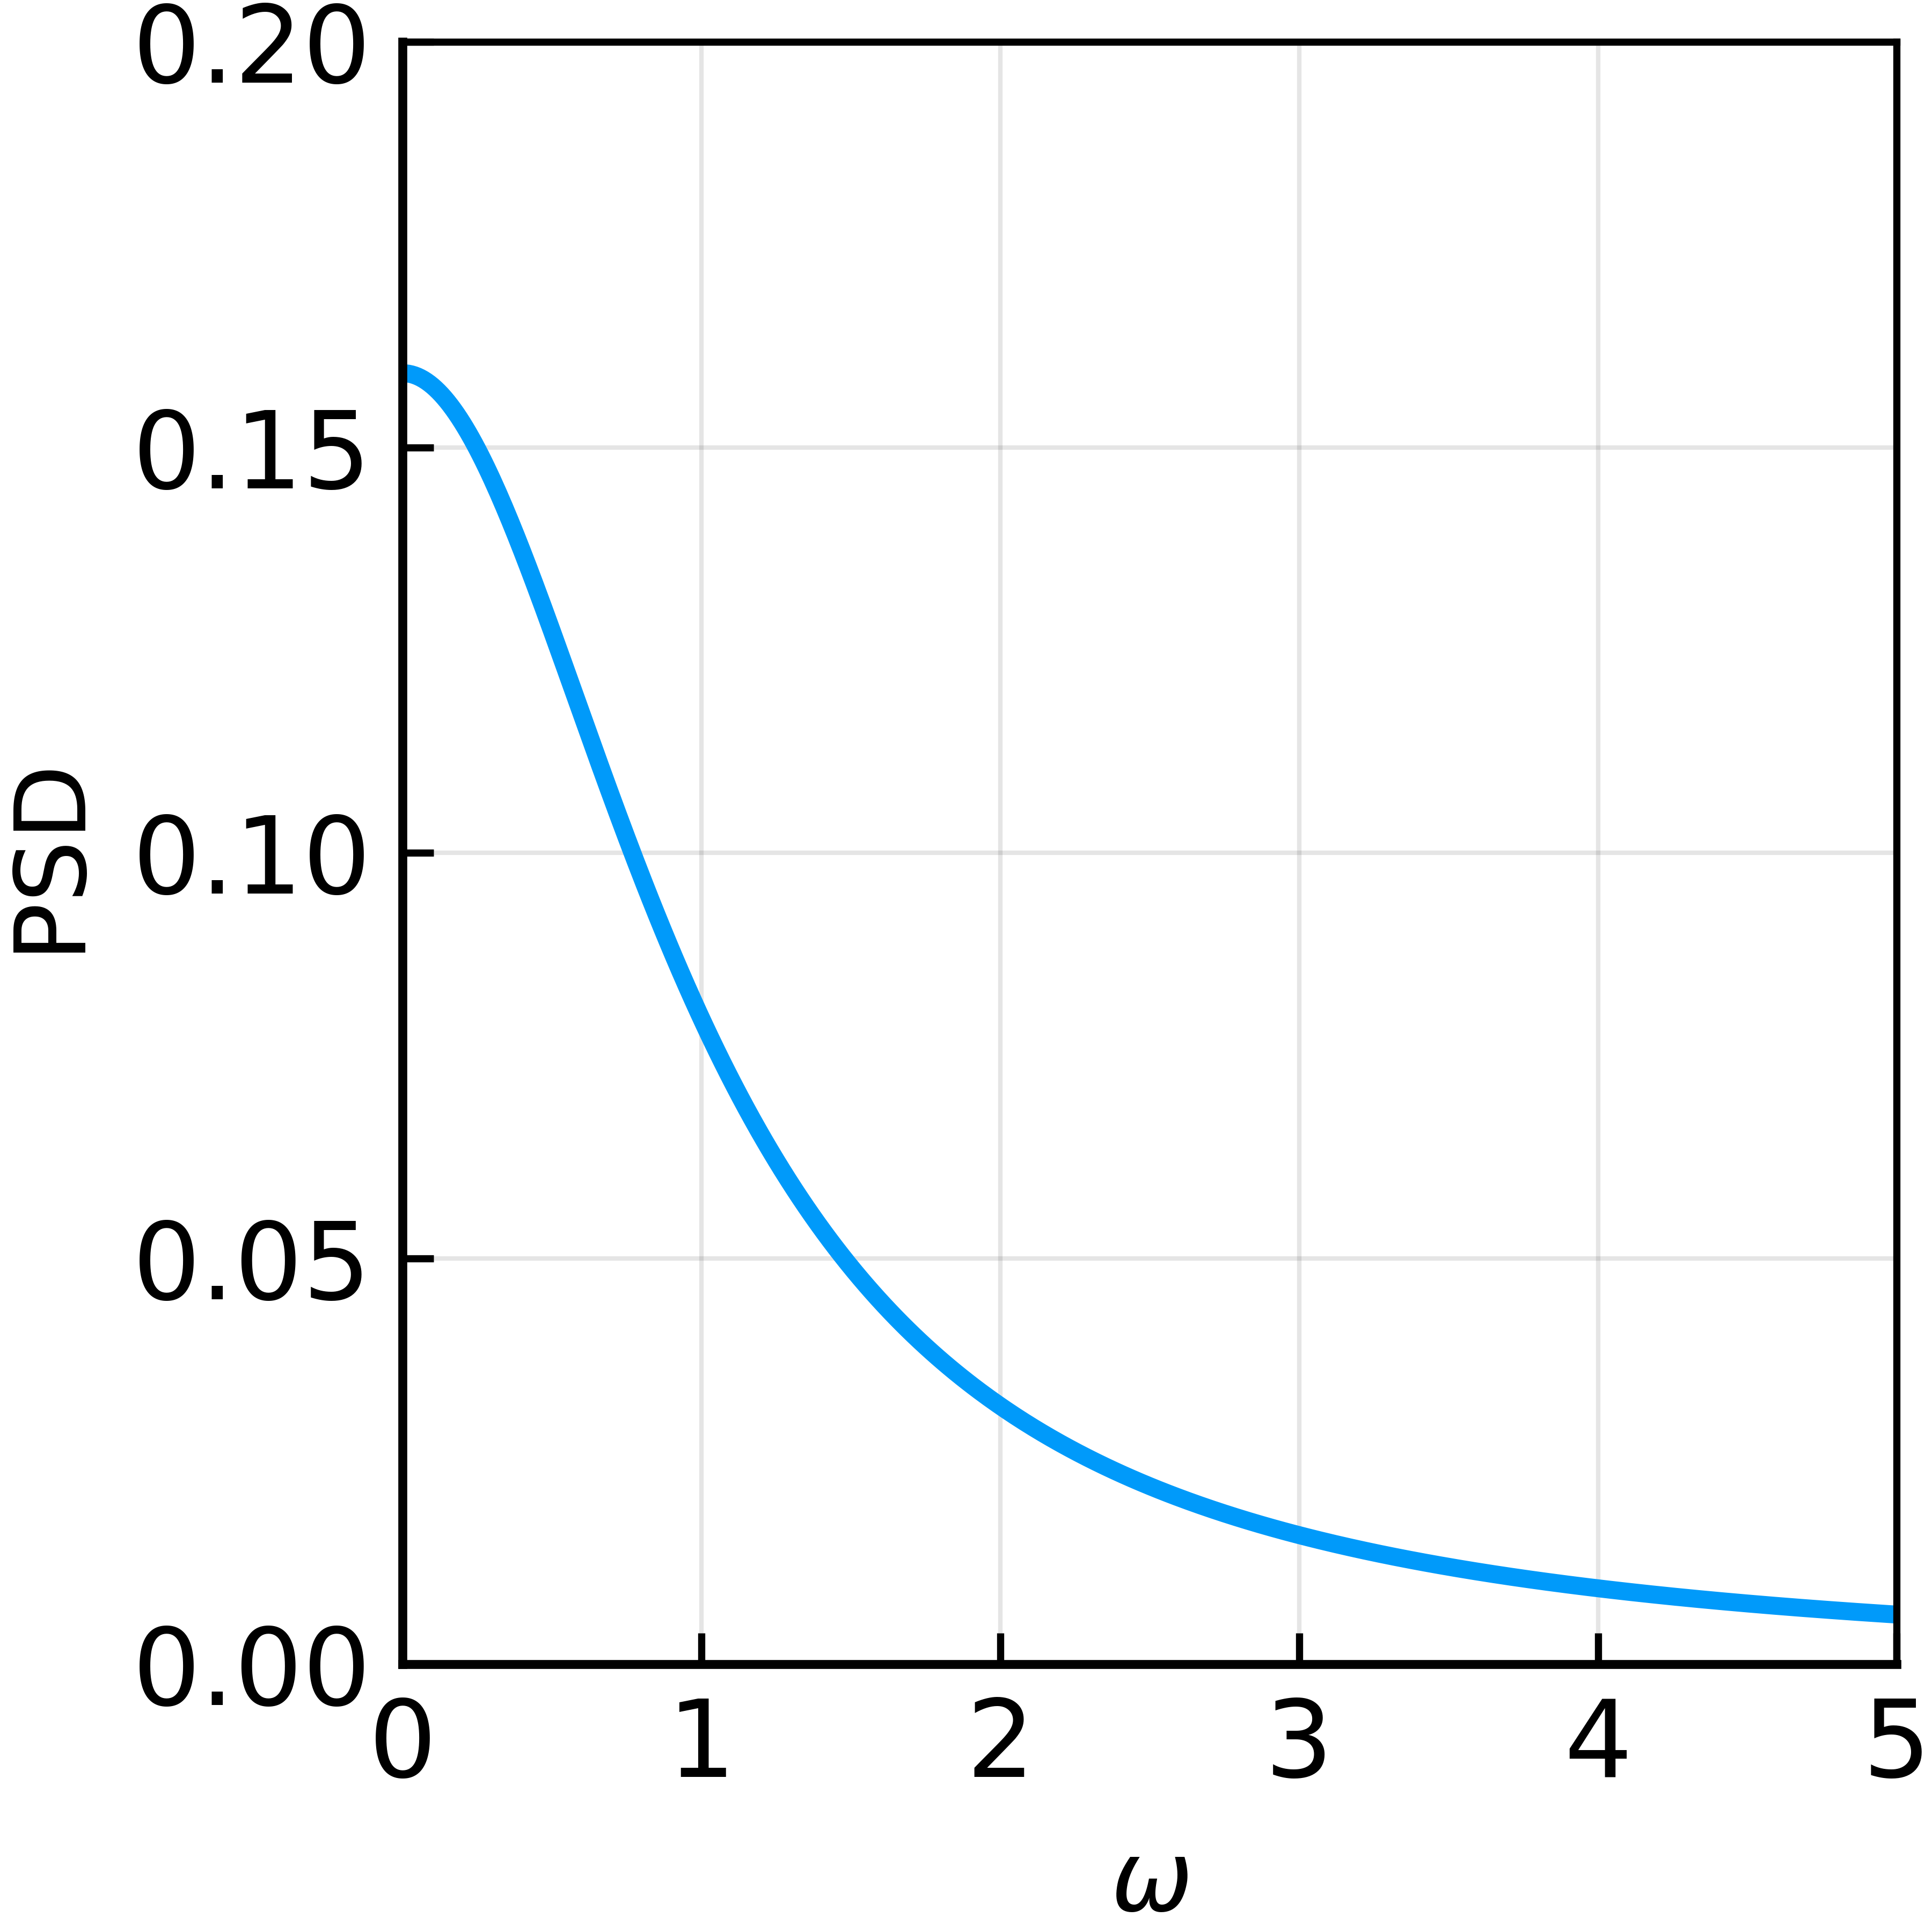
\includegraphics[width=.75\columnwidth]{ornstein_uhlenbeck_process_psd}

		\small{
			\textbf{Fig. 4:} Stationnary PSD of the OU process.
			}
	\end{minipage}

	\vspace{1cm}
\end{frame}

\begin{frame}[t, c]{Ornstein-Uhlenbek Process}{Autocorrelation function}
	\begin{minipage}{.48\textwidth}
		\begin{block}{\centering \textbf{Exercise}}
			Show that the AutoCorrelation Function (ACF) is given by
				$$
				G(\tau) = \frac{\sigma^2}{2\theta} e^{-\theta \vert \tau \vert}.
				$$
		\end{block}

		\bigskip

		\begin{itemize}
			\item Orstein-Uhlenbeck process gives rise to a random noise with finite-time correlation.
		\end{itemize}
	\end{minipage}%
	\hfill
	\begin{minipage}{.48\textwidth}
		\centering
		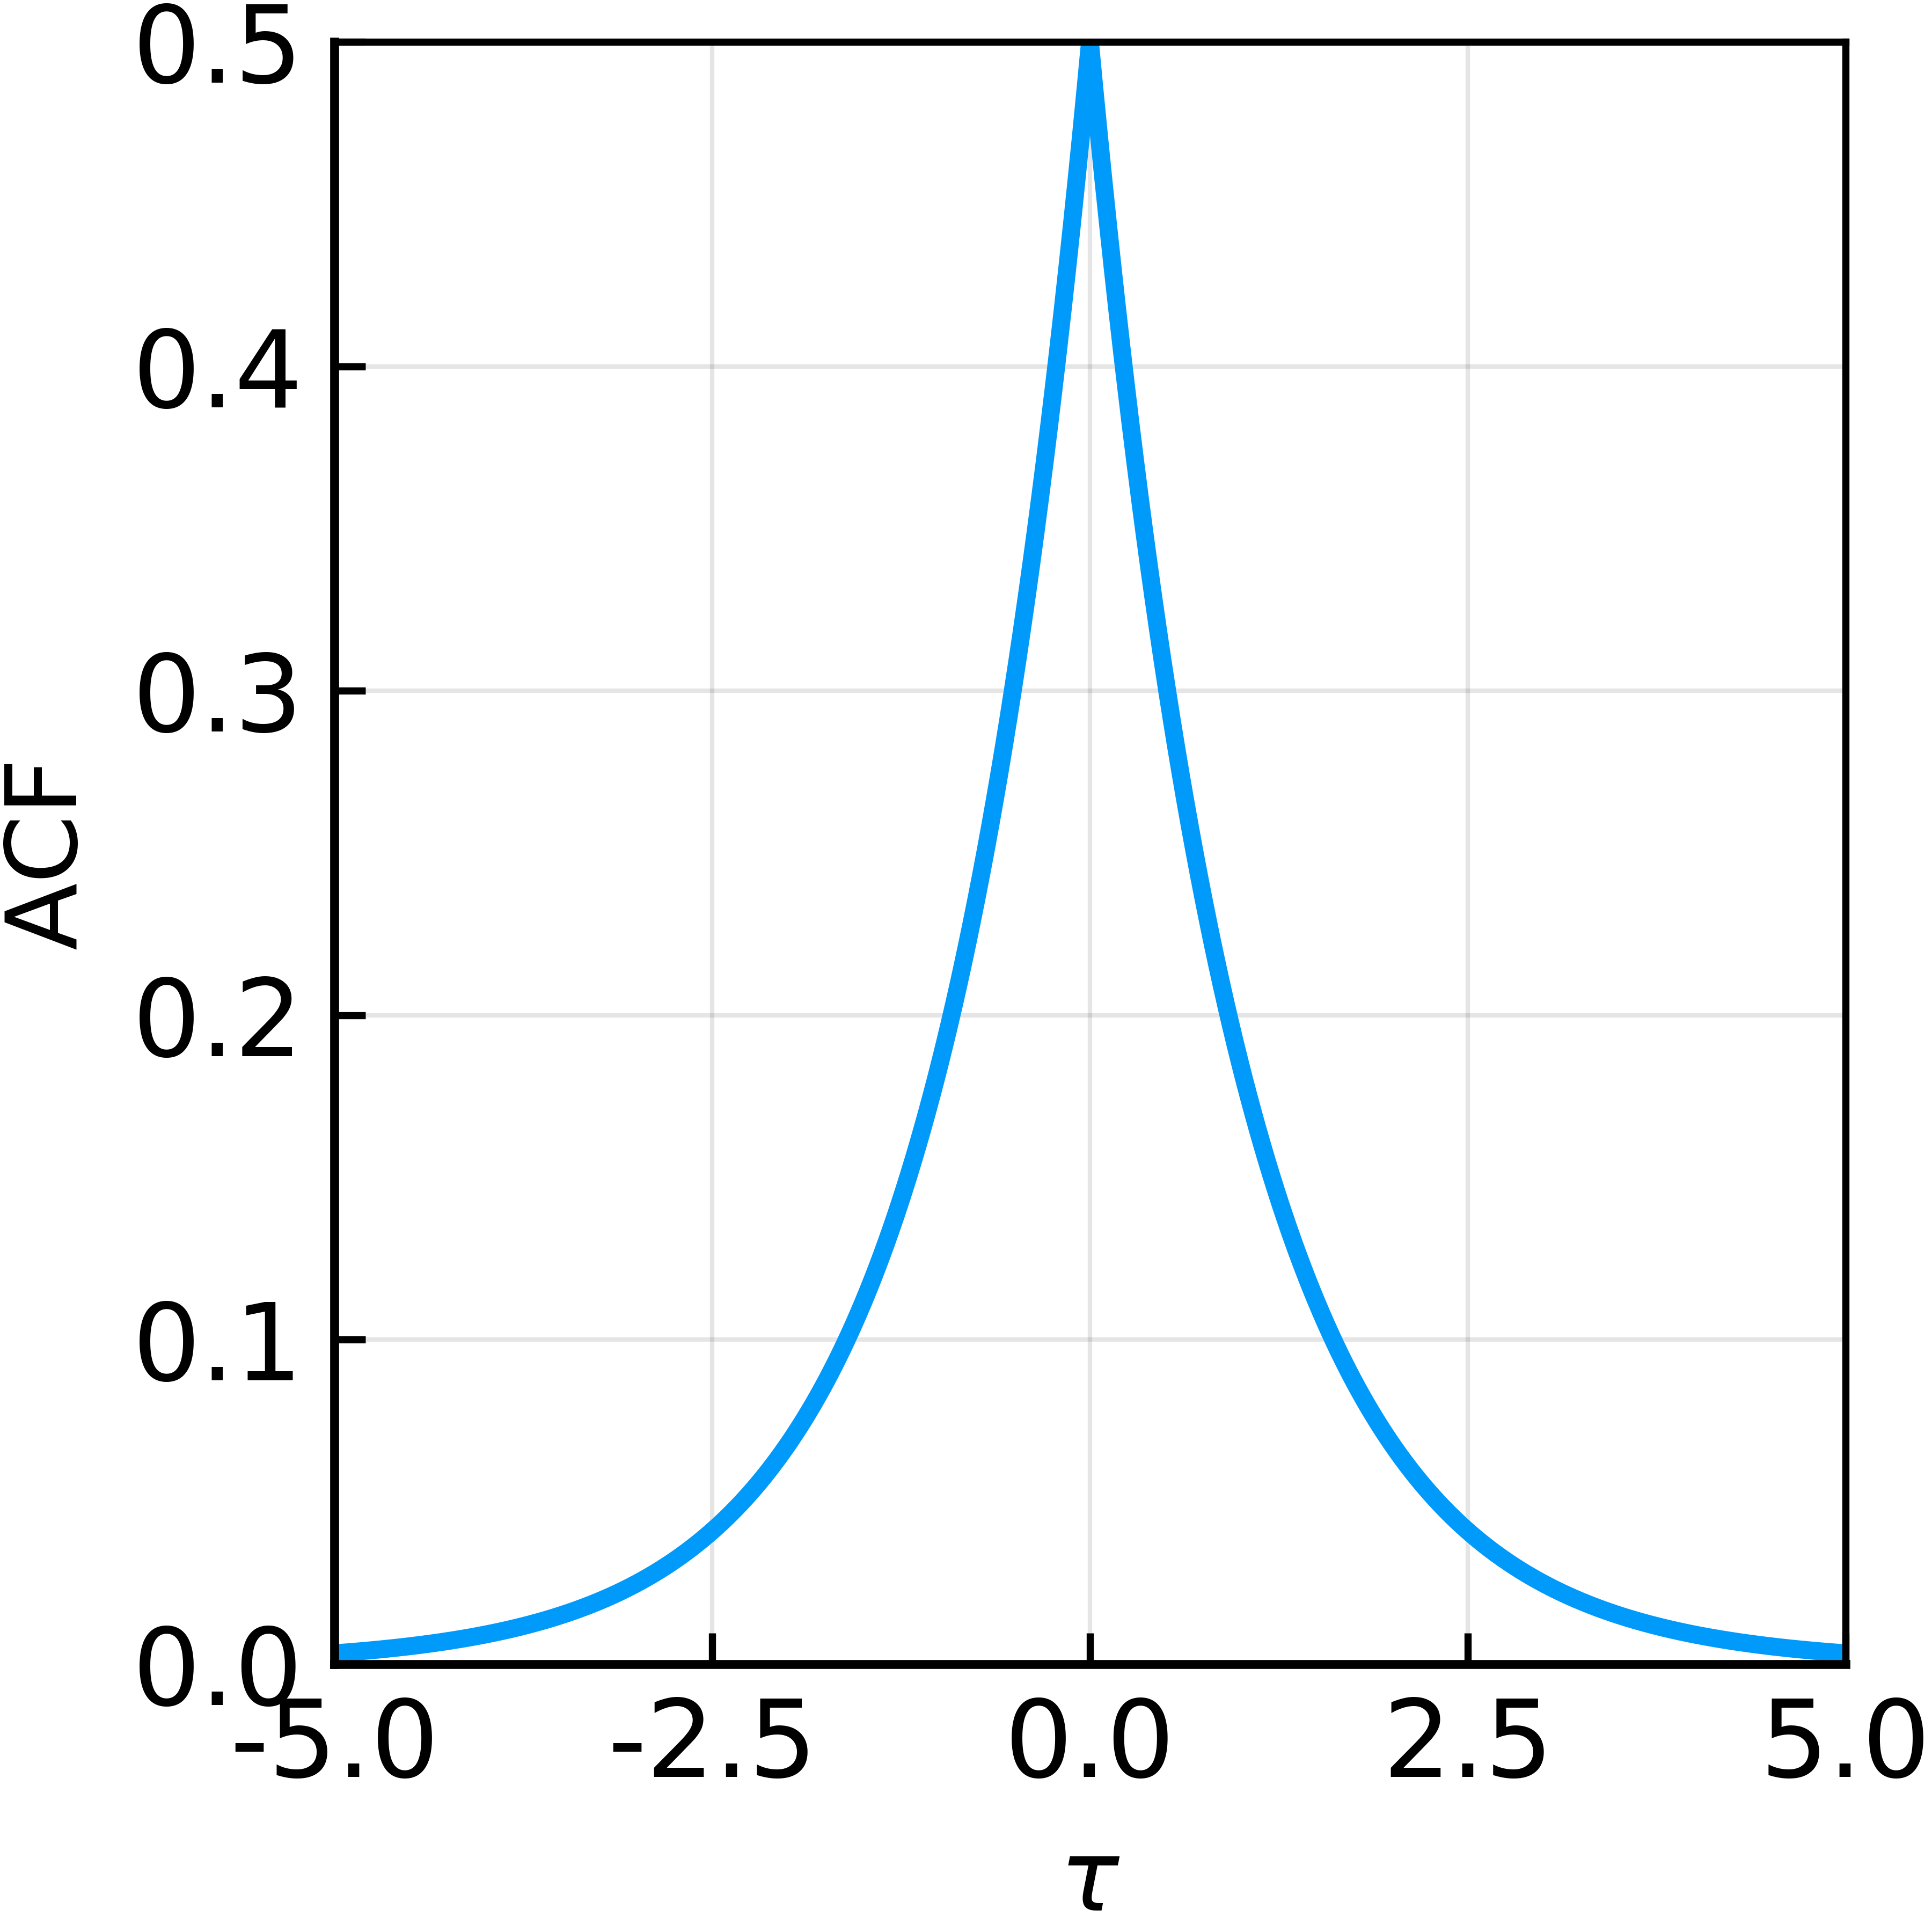
\includegraphics[width=.75\columnwidth]{ornstein_uhlenbeck_process_acf}

		\small{
			\textbf{Fig. 5:} Stationnary ACF of the OU process.
			}
	\end{minipage}

	\vspace{1cm}

\end{frame}

%-------------------------------------------------------------------------------
%										Brownian motion
%-------------------------------------------------------------------------------

\begin{frame}[t, c]{}
	\centering
	\vspace{1cm}

	{\Large \textbf{Brownian motion}}

	\bigskip

	{\textgre{\textbf{A prototype of stochastic dynamical system}}}

\end{frame}

\begin{frame}[t, c]{Brownian motion}{Prototype example}
	\begin{itemize}
		\item Brownian motion can be modeled as follows
		$$
		\begin{aligned}
			\dot{x} & = \frac{p}{m}, \\
			\dot{p} & = -\alpha p + \sqrt{2D} \eta
		\end{aligned}
		$$
		where $\alpha$ is the friction coefficient and $D$ characterizes the strength of the fluctuations.

		\medskip

		\item This stochastic dynamical system was the subject of one of Einstein's 1905 paper.
	\end{itemize}

	\vspace{1cm}
\end{frame}

\begin{frame}[t, c]{Brownian motion}{Monte-Carlo simualtions}
	\centering
	
\includegraphics[width=.8\textwidth]{brownian_motions}

	\textbf{Fig. 1:} Three different realizations of Brownian motion.

	\vspace{1cm}
\end{frame}

\begin{frame}[t, c]{Brownian motion}{Monte-Carlo simualtions}
	\centering
	\includegraphics[width=.8\textwidth]{brownian_motion_monte_carlo}

	\textbf{Fig. 2:} One hundred different realizations of Brownian motion.

	\vspace{1cm}
\end{frame}

\begin{frame}[t, c]{Brownian motion}{Monte-Carlo simualtions}
	\centering
	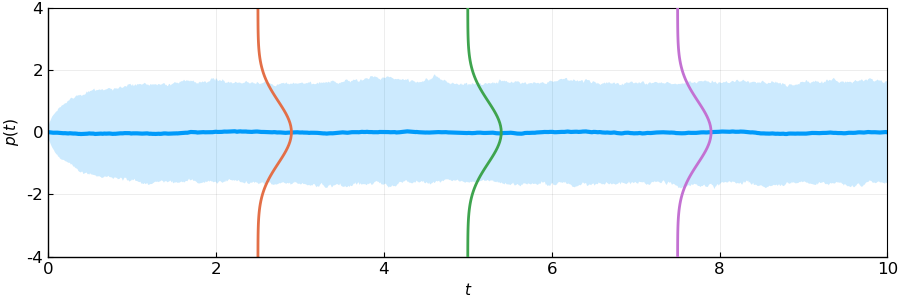
\includegraphics[width=.8\textwidth]{brownian_motion_monte_carlo_summary}

	\textbf{Fig. 3:} Evolution of the probability density function.

	\vspace{1cm}
\end{frame}

\begin{frame}[t, c]{Brownian motion}{Fokker-Planck equation}
	\begin{minipage}{.48\textwidth}
		\begin{itemize}
			\item The Fokker-Planck equation reads
			$$
			\frac{\partial \rho}{\partial t} = -\frac{\partial}{\partial x} \left( \frac{p}{m} \rho \right) + \frac{\partial}{\partial p} \left( \alpha p \rho + D \frac{\partial \rho}{\partial p} \right)
			$$
			where $\rho(x, p, t)$ is the probability density function.

			\medskip

			\item The stationnary PDF is given by
			$$
			\rho_s = \sqrt{\frac{\alpha}{2\pi D}} \exp \left( -\frac{\alpha p^2}{2D} \right).
			$$
			\begin{itemize}
				\item[$\hookrightarrow$] It is $x$-independent.
			\end{itemize}
		\end{itemize}
	\end{minipage}%
	\hfill
	\begin{minipage}{.48\textwidth}
		\centering
		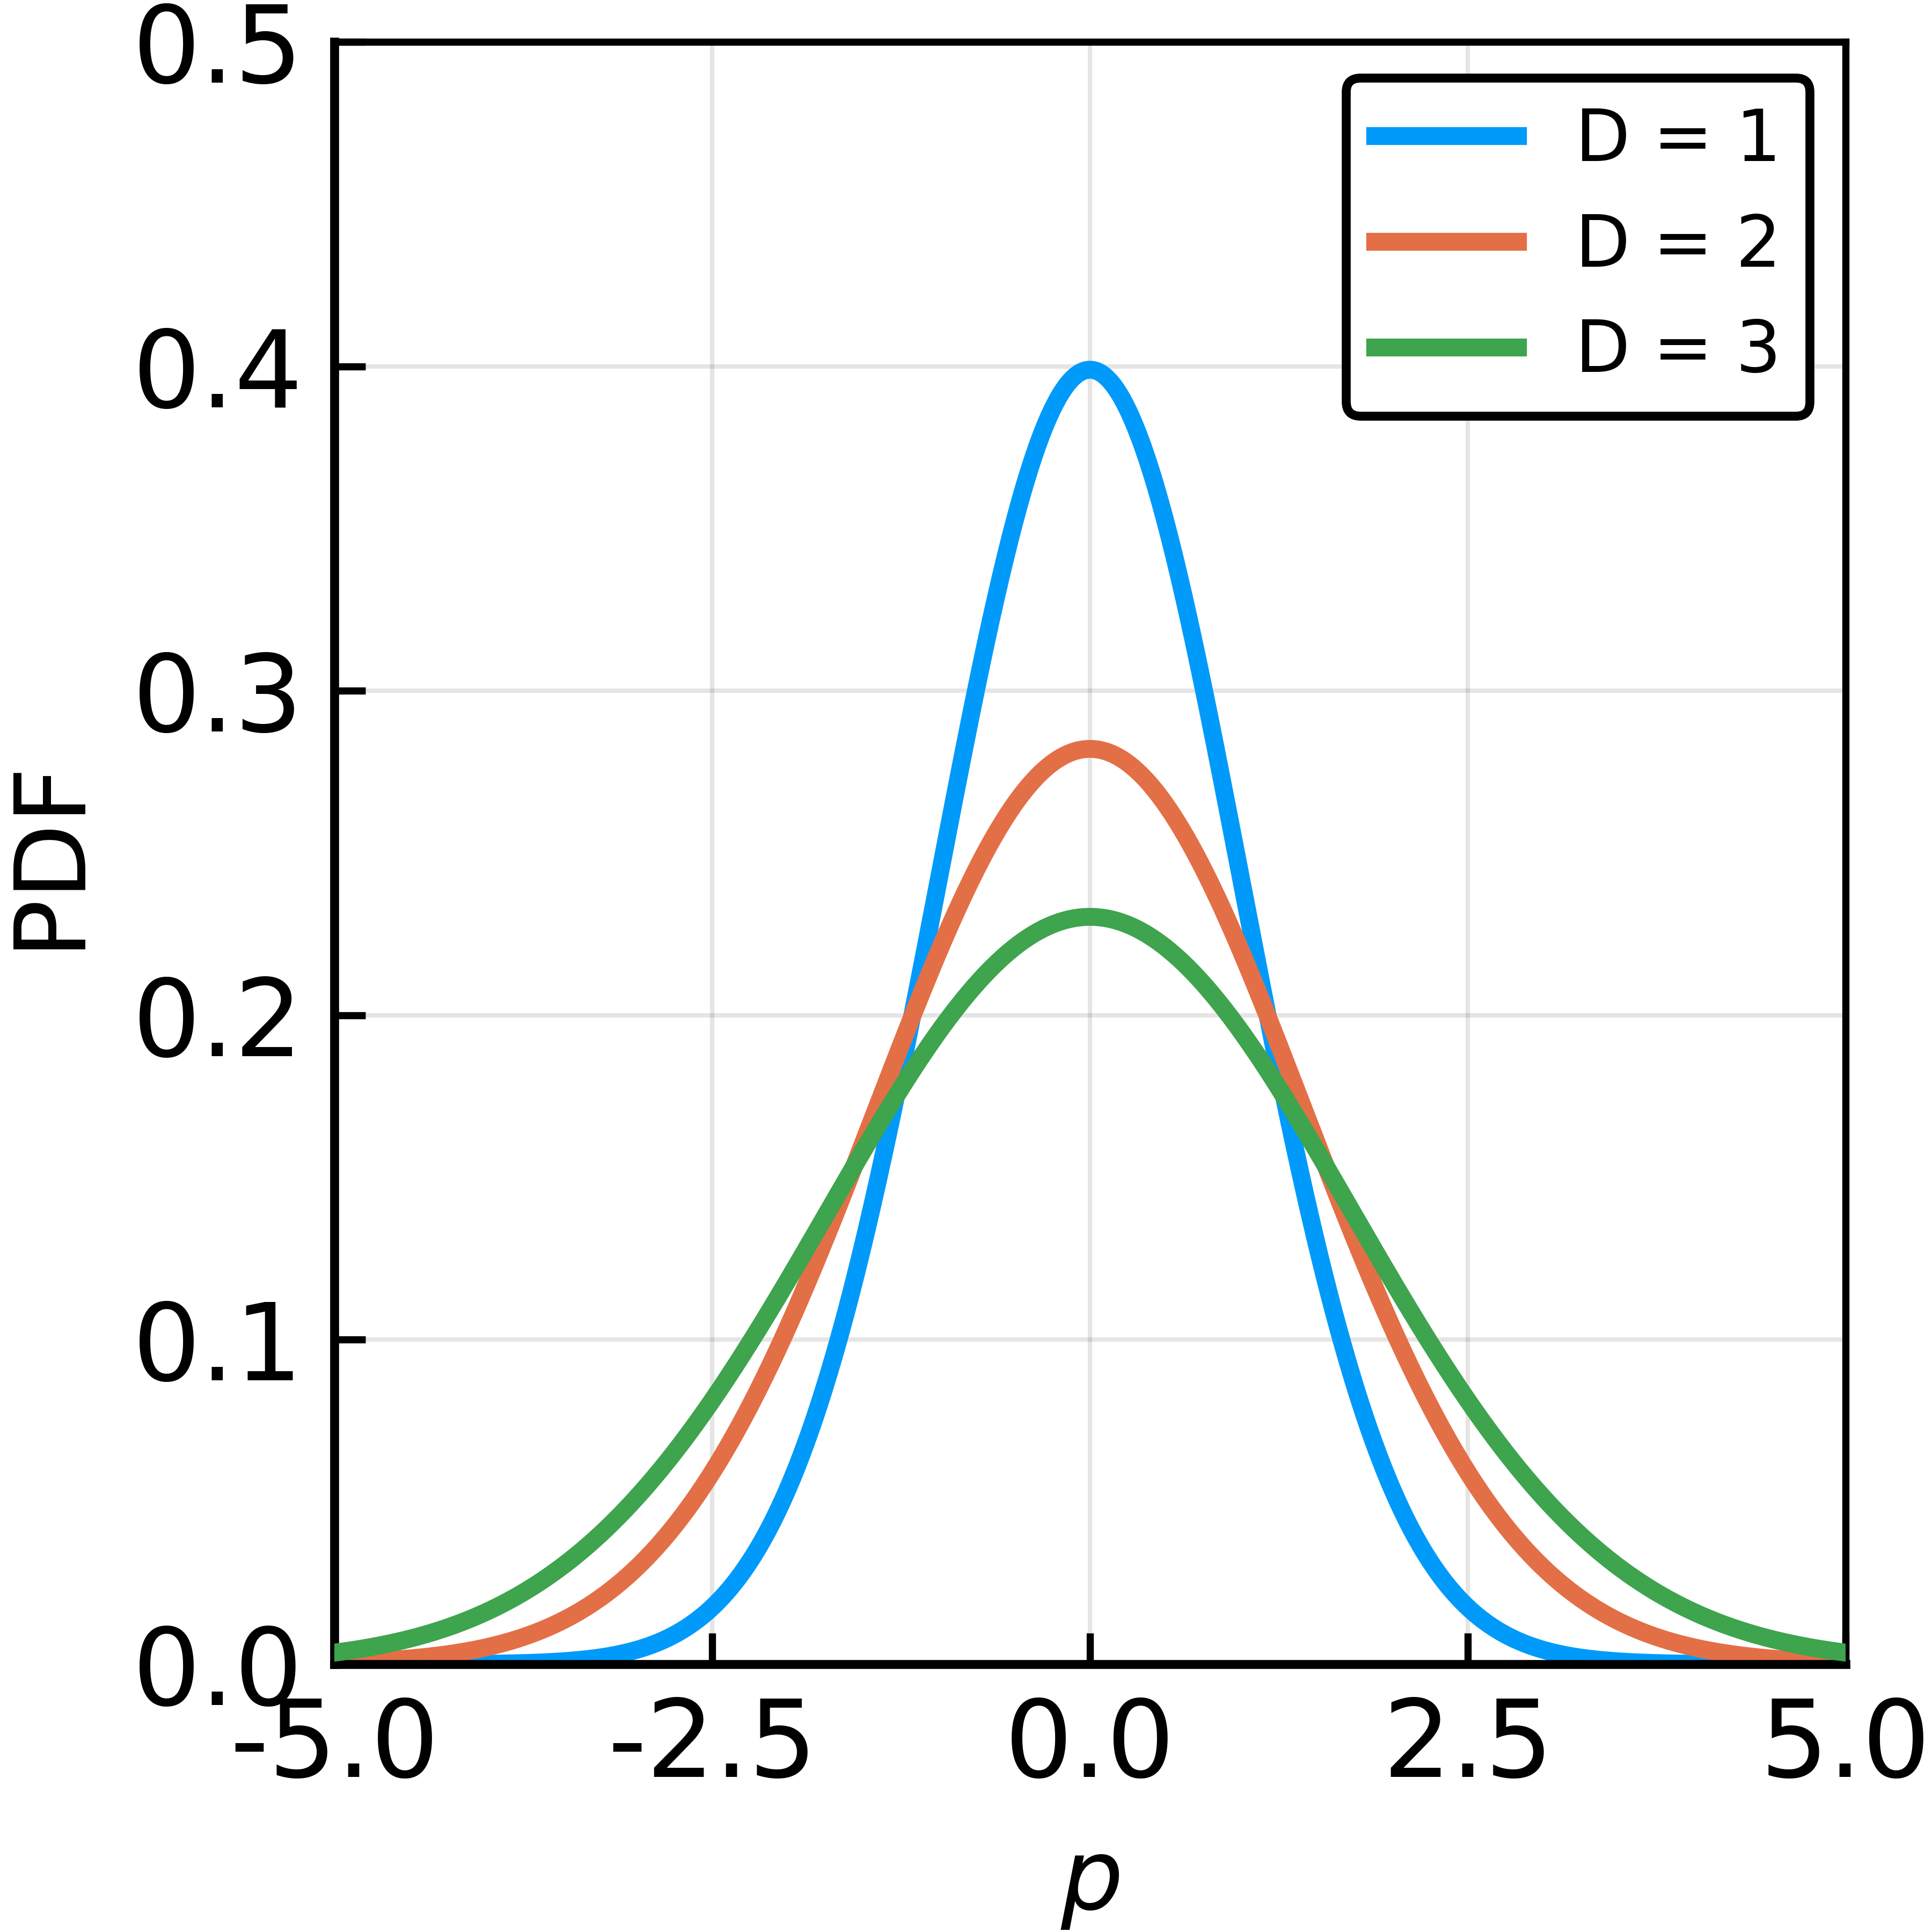
\includegraphics[width=.75\columnwidth]{brownian_motion_pdf}

		\small{
			\textbf{Fig. 4:} PDF of the Brownian motion.
			}
	\end{minipage}

	\vspace{1cm}
\end{frame}

\begin{frame}[t, c]{Brownian motion}{Back to physics}
	\begin{itemize}
		\item The Maxwell's velocity distribution at temperature $T$ is
		$$
		\rho_s(v) = \sqrt{ \frac{m}{2\pi kT} } \exp \left( -\frac{mv^2}{2kT} \right).
		$$

		\item This is consistent with the expression derived previously if we set
		$$
		D = \alpha m k T.
		$$
	\end{itemize}

	\begin{block}{\centering \textbf{Question}}
		\centering
		How to compute the diffusion coefficient of the particle?
		$$
		D_{\infty} = \lim_{t \to \infty} \frac{\langle \left( x(t) - x(0) \right)^2 \rangle}{2t}
		$$
	\end{block}

	\vspace{1cm}
\end{frame}

\begin{frame}[t, c]{Brownian motion}{Back to physics}
	\begin{itemize}
		\item We can use the Fokker-Planck equation to find $\langle x(t) \rangle$.
		\begin{equation}
			\begin{aligned}
				\frac{\partial \langle x(t) \rangle}{\partial t} & = \int x \frac{\partial \rho}{\partial t} \mathrm{d}x \mathrm{d}p \\
				& = \int x \left( -\frac{\partial}{\partial x} \left( \frac{p}{m} \rho \right) + \frac{\partial}{\partial p} \left( \alpha p \rho + D \frac{\partial \rho}{\partial p} \right) \right) \mathrm{d}x \mathrm{d}p \\
				& = \frac{ \langle p(t) \rangle }{m}.
			\end{aligned}
			\notag
		\end{equation}

		\item Similarly, we find the equations for $\langle p(t) \rangle$, $\langle x(t) p(t) \rangle$, $\langle p(t)^2 \rangle$ and $\langle x(t)^2 \rangle$.
	\end{itemize}

	\vspace{1cm}
\end{frame}

\begin{frame}[t, c]{Brownian motion}{Back to physics}
	\begin{itemize}
		\item We finally end up with the following set of ODEs.
		\begin{equation}
			\begin{aligned}
				\frac{\partial \langle x(t) \rangle}{\partial t} & = \frac{\langle p(t) \rangle}{m}, \\
				\frac{\partial \langle p(t) \rangle}{\partial t} & = -\alpha \langle p(t) \rangle, \\
				\frac{\partial \langle x(t) p(t) \rangle}{\partial t} & = \frac{\langle p(t)^2 \rangle}{m} - \alpha \langle x(t) p(t) \rangle, \\
				\frac{\partial \langle x(t)^2 \rangle}{\partial t} & = \frac{2\langle x(t) p(t) \rangle}{m}, \\
				\frac{\partial \langle p(t)^2 \rangle}{\partial t} & = -2\alpha \langle p(t)^2 \rangle + 2D.
			\end{aligned}
			\notag
		\end{equation}

		\item It is a closed system of linear equations for the first five moments of the PDF.
	\end{itemize}

	\vspace{1cm}
\end{frame}

\begin{frame}[t, c]{Brownian motion}{Back to physics}
	\begin{itemize}
		\item The analytical solutions are given by
		\begin{equation}
			\begin{aligned}
				\langle p(t) \rangle & = p_0 e^{-\alpha(t-t_0)} \\
				\langle p(t)^2 \rangle & = \frac{D}{\alpha} \left( 1 - e^{-2\alpha(t-t_0)} \right) + p_0^2 e^{-2\alpha(t-t_0)}, \\
				\langle x(t) \rangle & = x_0 + \frac{p_0}{\alpha m} \left( 1 - e^{-\alpha(t-t_0)} \right), \\
				\langle x(t) p(t) \rangle & = \frac{D}{\alpha^2m} - \left( \frac{p_0^2}{\alpha m} - \frac{D}{\alpha^2 m} \right) e^{-2\alpha(t-t_0)} + \left( (xp)_0 - \frac{2D}{\alpha^2m} + \frac{p_0^2}{\alpha m} \right) e^{-\alpha(t-t_0)},\\
				\langle x(t)^2 \rangle & = \frac{2Dt}{(\alpha m)^2} + C_1 e^{-\alpha (t-t_0)} + C_2 e^{-2\alpha(t-t_0)}.
			\end{aligned}
			\notag
		\end{equation}

		\item We can now work out the diffusion coefficient $D_{\infty}$.
	\end{itemize}

	\vspace{1cm}
\end{frame}

\begin{frame}[t, c]{Brownian motion}{Back to physics}
	\begin{itemize}
		\item Finally, we end up with the diffusion coefficient
		$$
		D_{\infty} = \frac{D}{(\alpha m)^2} = \frac{kT}{\alpha m}.
		$$

		\medskip

		\item We thus have $\langle \left( x(t) - x(0) \right)^2 \rangle \propto t$, i.e.\ the distance travelled by a particle over time $t$ is proportional to $\sqrt{t}$.

		\medskip

		\item Einstein then relates the diffusion constant $D_{\infty}$ to physically measurable quantities, enabling the experimental determination of Avogaro's number and therefore the size of molecules.
	\end{itemize}

	\vspace{1cm}
\end{frame}

\end{document}
